% -*- coding: utf-8 -*-
%%\mainmatter
\cleardoublepage
\chapter{Arquitectura}
\thispagestyle{fancy}
%%\setcounter{page}{32}

\section{\uppercase{Introducción}}

\begin{figure}[ht]
    \begin{center}
        
\includegraphics[scale=0.5]{src/img/fs-logo.png}
        \caption[Logo de Free Station]
          {Logo de Free Station}
    \end{center}
\end{figure}

\drop{F}{}reeStation o «Librenería» es un software para centros o puntos de
acceso de distribución de información de software libre orientado a centros de enseñanza y
universidades.

El sistema esta compuesto por un armario de diseño con un ordenador empotrado
con pantalla táctil y una cámara para reconocer movimientos y gestos. En dicho
dispositivo se encuentra un software cliente que alberga repositorios de
software modularizables configurados por el centro de enseñanza o universidad,
con software como imágenes de distribuciones GNU/Linux, software específico
para los alumnos o aplicaciones educativas para interactuar con el
dispositivo.

El dispositivo puede incorporar una unidad de CD-ROM y USB con la que el
usuario/docente puede grabar los datos proporcionados por el sistema en pocos
segundos y hacerse una copia de todo software gratuito y opensource disponible.

Además el sistema cuenta con otra aplicación servidor, que distribuye
diariamente a todos los clientes el software y los módulos actualizados.

\section{\uppercase{Descripción general}}

La arquitectura de FreeStation está principalmente basada en el modelo
cliente-servidor. Cada componente es modularizable y fácilmente
personalizable. Su diseño esta pensado para no requerir especiales
conocimientos técnicos para su uso y administración diarios.

FreeStation o «Librenería» es el software cliente y servidor para
la organización de puntos de acceso e interés de software libre catalogado y
modularizado en estaciones libres.

\begin{figure}[ht]
    \begin{center}
        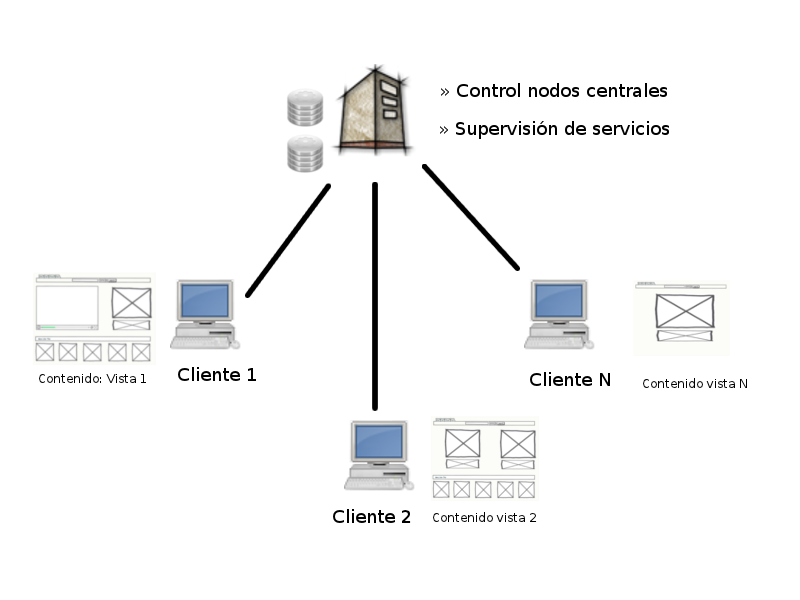
\includegraphics[scale=0.5]{src/img/infraestructure.png}
        \caption[Arquitectura propuesta]
          {Arquitectura propuesta}
          \label{arquitectura}
    \end{center}
\end{figure}

La arquitectura propuesta en la figura \ref{arquitectura} habilita un nodo principal
servidor que dispone de métodos de interacción para la supervisión sencilla del servidor
además del control de los nodos centrales restantes.
\newpage

\begin{figure}[ht]
    \begin{center}
        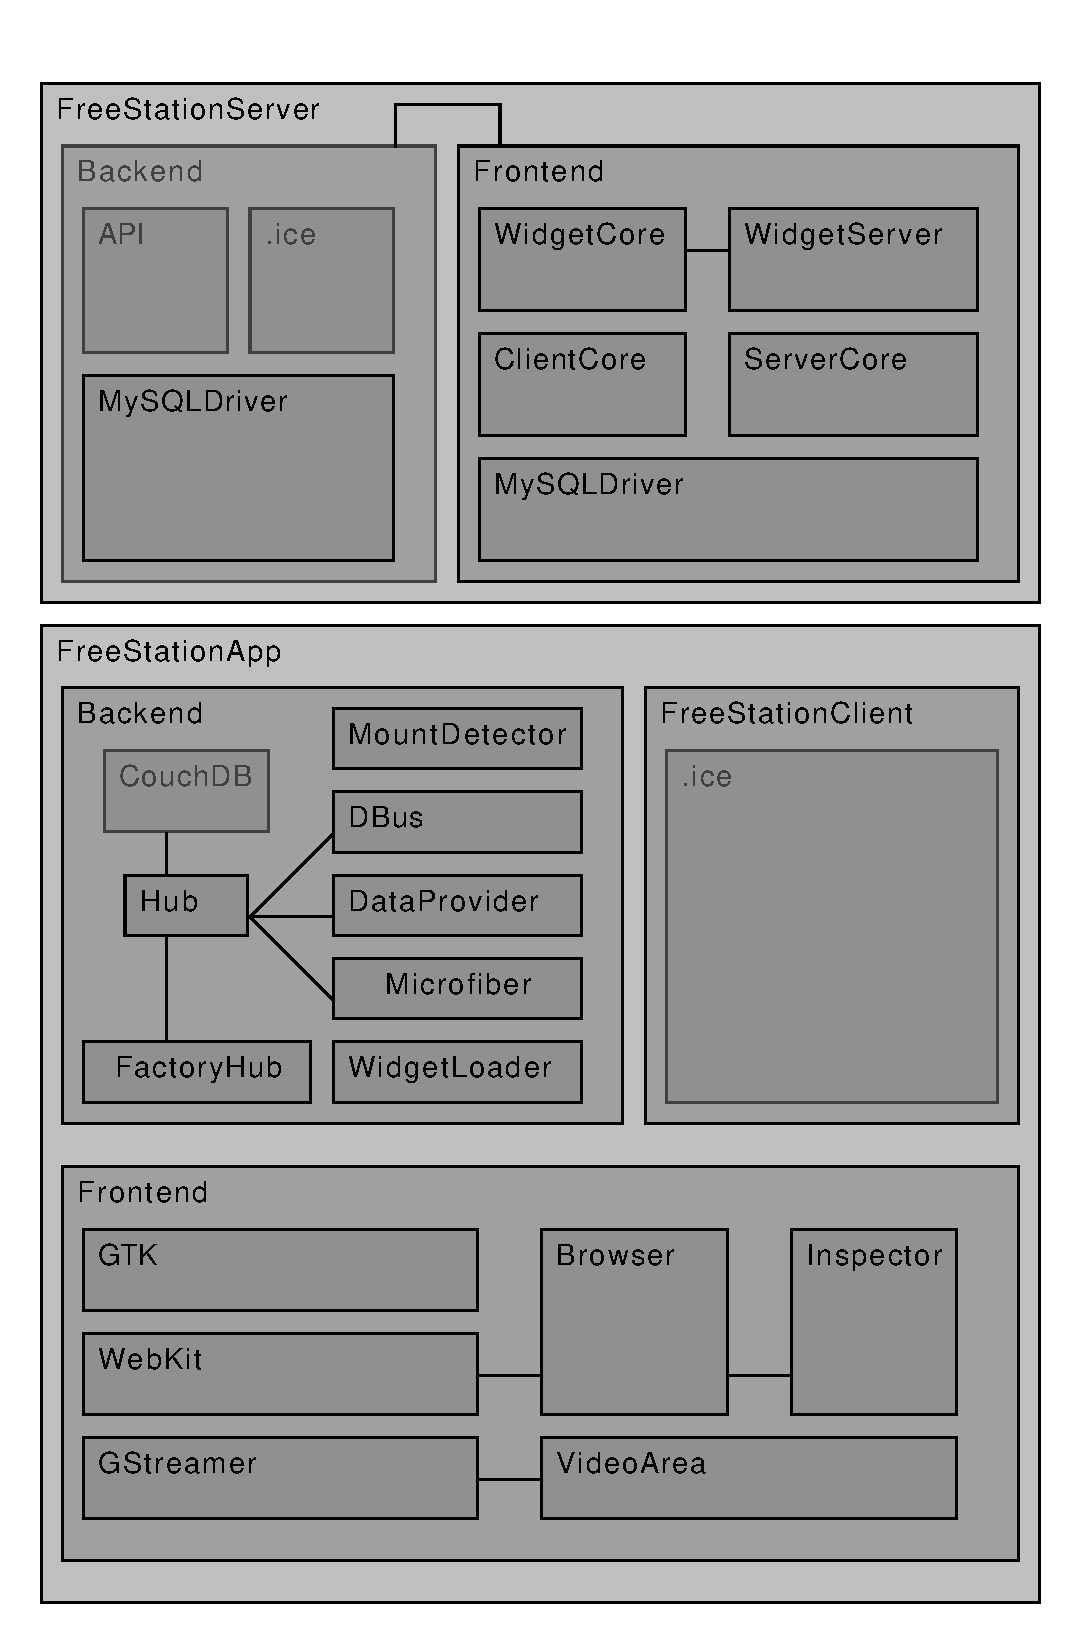
\includegraphics[width=320px]{src/img/diagrams/freestation-full-architecture-diagram.pdf}
        \caption[Diagrama de la arquitectura general y subsistemas]
          {Diagrama de la arquitectura general y subsistemas}
          \label{fig:arqgeneral}
    \end{center}
\end{figure}

El servidor actúa como replica de la información de consulta y difunde o distribuye
los contenidos en los nodos clientes solicitados en los que el usuario dispone de una
interfaz para su uso.

La figura ~\ref{fig:arqgeneral} muestra un diagrama de la arquitectura
general y subsistemas que indican los módulos que lo componen de forma general.
En posteriores secciones serán detallados más profundamente.

\newpage

\section{\uppercase{Arquitectura del servidor}}

El servidor FreeStation funciona sobre una pila de software consistente en
varias tecnologías y componentes. El servidor es el encargado de
administrar la comunicación con cada cliente.

\subsection{Descripción general}

El servidor dispone de un un panel de interfaz (\acs{GUI}\label{acro:GUI})
basado en PHP y Javascript.

\begin{figure}[h]
    \begin{center}
        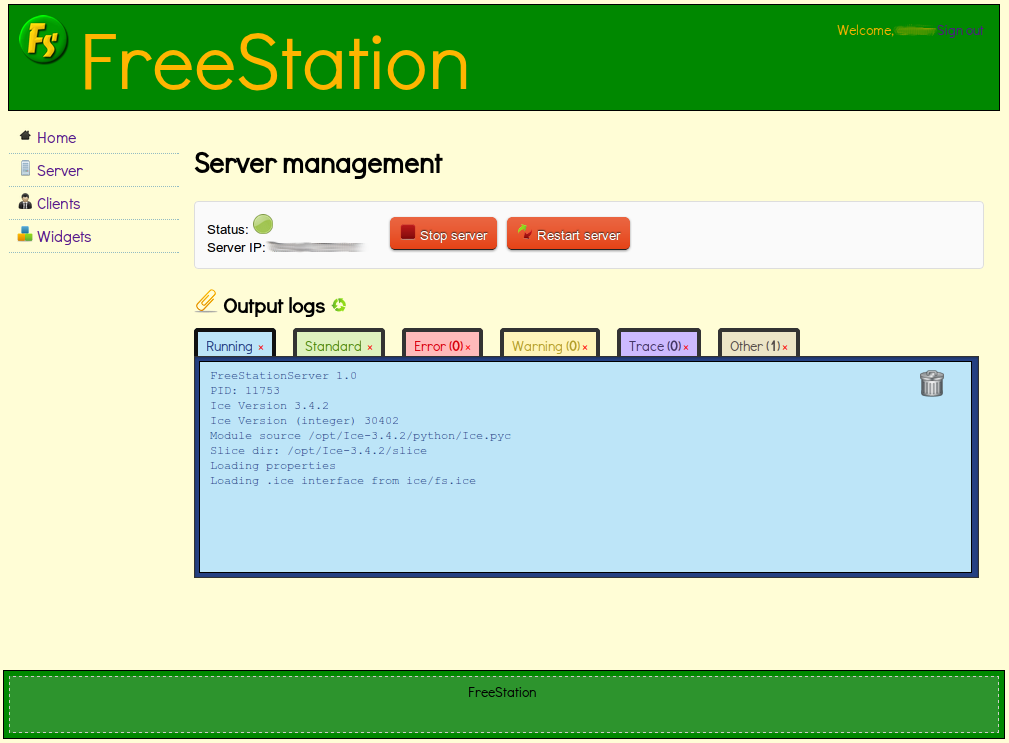
\includegraphics[scale=0.45]{src/img/freestation-server-gui.png}
        \caption[FreeStation Server Webserver GUI] {FreeStation Server Webserver GUI}
        \label{fig:serverGUI}
    \end{center}
\end{figure}

\newpage

Como se puede observar en ~\ref{fig:serverGUI}, existen funciones de
\emph{iniciar/apagar/reiniciar} el servidor desde la interfaz y ver el estado
real del mismo con un listado de registro de salidas de errores útiles. Mediante estos
registros es posible analizar y diagnosticar cualquier actividad o evento en el
servidor o errores que se produzcan.

Asimismo, permite fácilmente la administración de tareas sencillas para
administrar y configurar tareas comunes para un número elevado de clientes con
POIs.

\subsection{Composición de capas}

Bajo la interfaz gráfica del servidor web, se ejecuta un proceso demonio
que actúa como backend y que esta basado en Python.

De esta forma, cada acción en la interfaz web se traduce como una tarea
interna para el backend que es despachada de forma rápida.

El backend puede realizar comunicaciones asíncronas con los clientes. Para
ello, se basa en \acs{ICE}\label{acro:ICE} (Internet Comunication Engine de
ZeroIce).

Esto permite transferir grandes conjuntos de información a un gran número de
clientes con un sólo servidor de una forma fiable y robusta.

Tanto frontend como backend disponen de una capa de persistencia en la que
almacenar los datos no volátiles de operaciones. En esta capa, se encuentra un
servidor de base de datos mysql, que es el encargado de almacenar de forma
persistente los datos (Mysql Storage).

De esta forma los datos pueden ser escritos de forma concurrente por el backend
o el frontend sin generar inconsistencias en los datos.
\newpage
Los datos accedidos por el backend son un conjunto limitado a datos internos
para operar con clientes, mientras que los datos accedidos por el frontend se
limitan a la configuración básica de administración.

Toda configuración que sea necesaria consultar con posterioridad por el
servidor es almacenada en la capa persistente.

Subconjuntos de esta configuración es transmitidas a
los clientes que la requieran para desplegar sus ejecuciones.

Por ejemplo, es posible visualizar un conjunto de los clientes actuales
manejados por el servidor y las estadísticas de los mismos:

\begin{figure}[ht]
    \begin{center}
        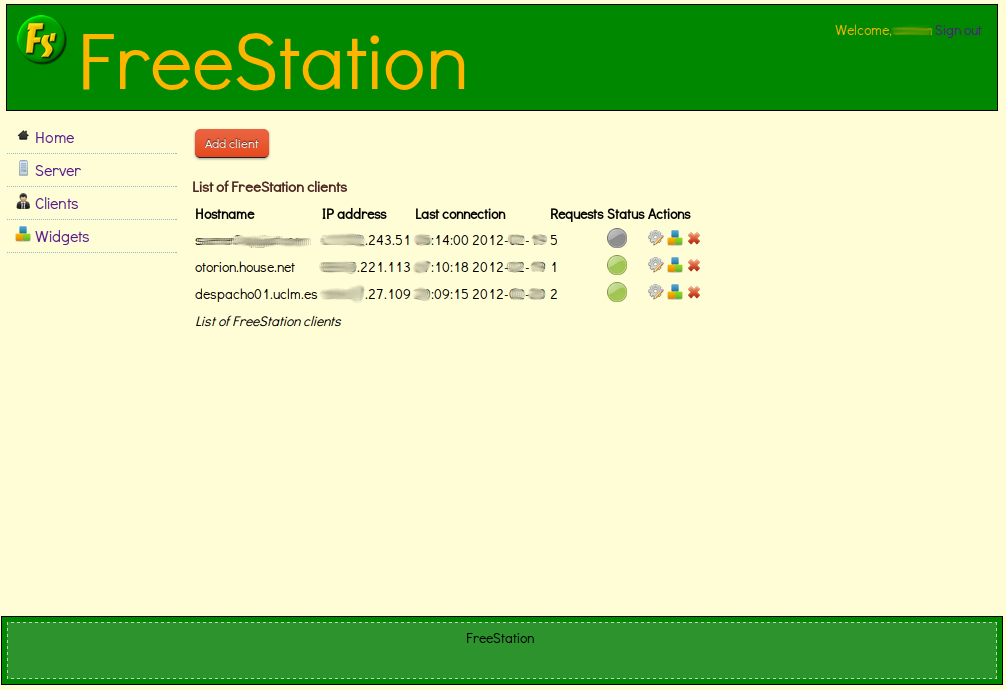
\includegraphics[scale=0.45]{src/img/freestation-server-clients.png}
        \caption[FreeStation Server
        GUI - Listado de clientes] {FreeStation Server GUI - Listado de clientes}
        \label{client_list}
    \end{center}
\end{figure}

\newpage

Como se muestra en el listado de la figura \ref{client_list} para cada cliente
se visualizan estadísticas de:

\begin{itemize}
  \item Hostname (el nombre de la máquina cliente)
  \item Direción IP en formato IPv4.
  \item Tiempo registrado de la última conexión realizada
  \item Número de peticiones realizadas (acumuladas) en total por el cliente.
  \item Iconos de acción para configuración
\end{itemize}

Los iconos de acción permiten añadir/eliminar/editar clientes y todos los datos
derivados para ese cliente que estén vinculados serán actualizados de forma
asíncrona.

\section{\uppercase{Arquitectura del cliente}}

El modelo cliente se ejecuta normalmente sobre un ordenador de escritorio o
terminal que servirá como referente para un POI (Point Of Interest).

\begin{figure}[hb]
    \begin{center}
        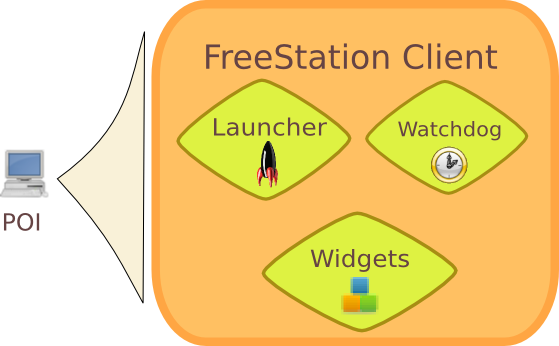
\includegraphics[scale=0.8]{src/img/client-diagram.png}
        \caption[Componentes de arquitectura cliente]
          {Componentes de arquitectura cliente}
    \end{center}
\end{figure}

\newpage

Para obtener la configuración general, el cliente contacta con su servidor
central y el cliente recibe la configuración general y composición de widgets
desde el servidor central y este carga deacuerdo a sus especificaciones.

Esta configuración sólo será recibida si el cliente esta autorizado en el
servidor y si este esta habilitado en el servidor.

\begin{figure}[hb]
    \begin{center}
        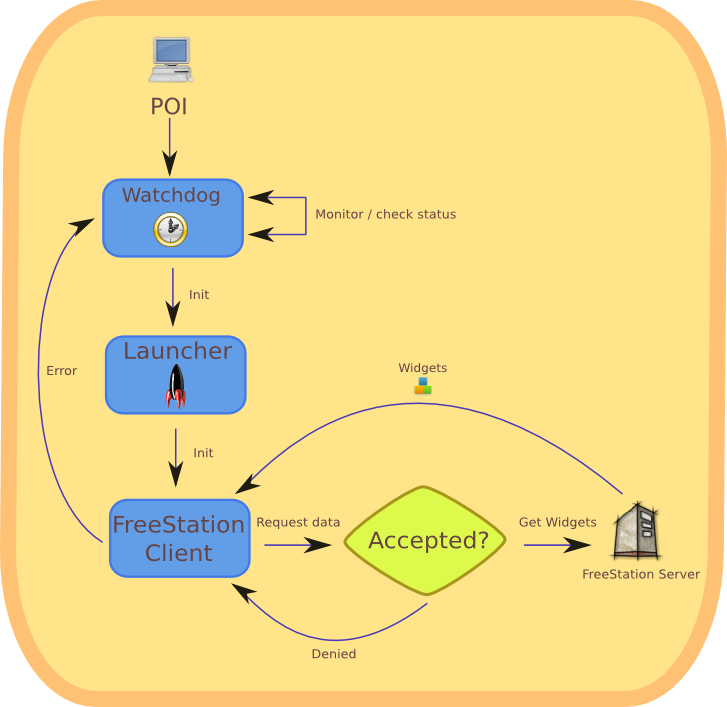
\includegraphics[scale=0.8]{src/img/client-flow-diagram.png}
        \caption[Diagrama de flujo - Cliente] {Diagrama de flujo - Cliente}
        \label{fig:flowclient}
    \end{center}
\end{figure}

En el diagrama de flujo de la figura ~\ref{fig:flowclient} puede observarse
dicha interacción.

\newpage
El modelo cliente esta programado en el lenguaje Python, por ser un lenguaje
rápido y de prototipado, normalmente muy útil para realizar interfaces de
escritorio bajo la plataforma GNU/Linux.

Un cliente se ejecuta sólo en un \acs{POI}\label{acro:POI} y periódicamente
consulta al servidor para recibir actualizaciones de contenidos o información. Los
clientes necesitan las especificaciones para configurar los widgets o
componentes y los datos asociados para cada widget.

Un POI debe ser accesible continuamente para los usuarios que lo requieran y
por ello debe ser robusto ante fallos y minimizar todos los riesgos posibles de
seguridad en acceso al mismo y sus componentes.

El cliente dispone de un programa lanzador «launcher» que inicia el programa
principal y se encarga de monitorizar en intervalos de tiempo regulares
mediante un programa watchdog la aplicación del modelo cliente y asegurarse de
que siga completamente funcional.

En el momento que se produce algún fallo crítico o se compromete el modelo
cliente, el watchdog reinicia la aplicación y establece los valores
funcionales sin que se adviertan problemas para el usuario.

\section{\uppercase{Arquitectura de widgets}}

\subsection{Definición de widget y su aplicación}

Un widget en la terminología de FreeStation es un elemento abstracto que lleva a
cabo operaciones atómicas sobre un dominio reducido de actuación y que provee
una comunicación para manejar la información de los datos que almacena el
widget.

Un widget esta representado simbólicamente con el icono de la figura
~\ref{fig:widgeticon}.

\begin{figure}[ht]
    \begin{center}
        
\includegraphics[width=16px]{src/img/widgets.png}
        \caption[Icono de representación para widgets] {Icono de representación para widgets}
        \label{fig:widgeticon}
    \end{center}
\end{figure}

\newpage

En los datos de un widget puede encontrarse la configuración del widget que será
tratada por el cliente.

\begin{figure}[ht]
    \begin{center}
        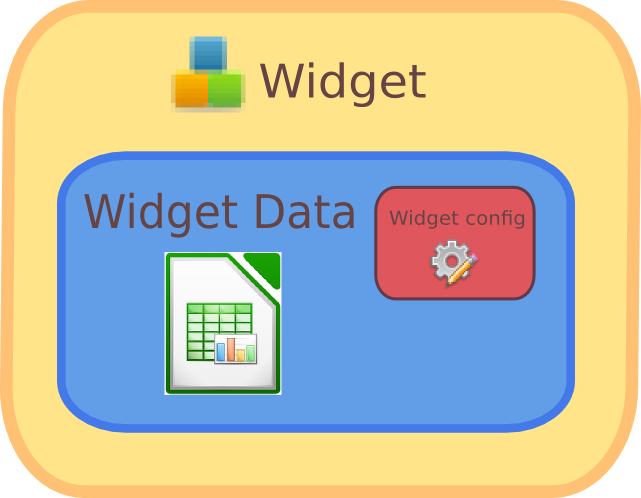
\includegraphics[scale=0.7]{src/img/widget-container.png}
        \caption[Contenedor Widget - Composición] {Contenedor Widget -
        Composición}
    \end{center}
\end{figure}

Para operaciones complejas un widget puede asociarse con más widgets para
llevar a cabo tareas sofisticadas o simplemente comunicar datos con otros
widgets. Los widgets son sólo ejecutados en el cliente, pero todos ellos son
únicamente configurados desde el servidor.

\subsection{Modelo orquesta}

La configuración de widgets entre cliente-servidor describe lo que se
conoce como modelo orquesta\cite{RoS04} donde un servidor actúa como
dirigente/administrador (coreógrafo) de un conjunto de
clientes con widgets que actúan como un coro de orquesta.

Esta situación se traduce en la restricción de que un cliente sólo puede
comunicarse con el servidor y no tiene permitido comunicarse con otros
clientes.

\newpage

El inconveniente de este modelo arquitectural, es que puede ser fácilmente
vulnerable a fallo al contar con un único punto de fallo
(\acs{SPOF}\label{acro:SPOF}).

Por ello, esta planeado en un futuro, añadir la capacidad de replicación de
varios servidores master como método failover (antifallo) y que estos
sincronicen sus propios datos entre servidores masters replicando la
información.

\subsection{Listado de widgets iniciales}

En un servidor, se dispone de un listado de widgets iniciales
para configurar un cliente. El propósito del mismo es ofrecer una base inicial
para configuración mínima. El usuario puede disponer de un mayor número si los
incorpora en el desarrollo.

\begin{figure}[ht]
    \begin{center}
        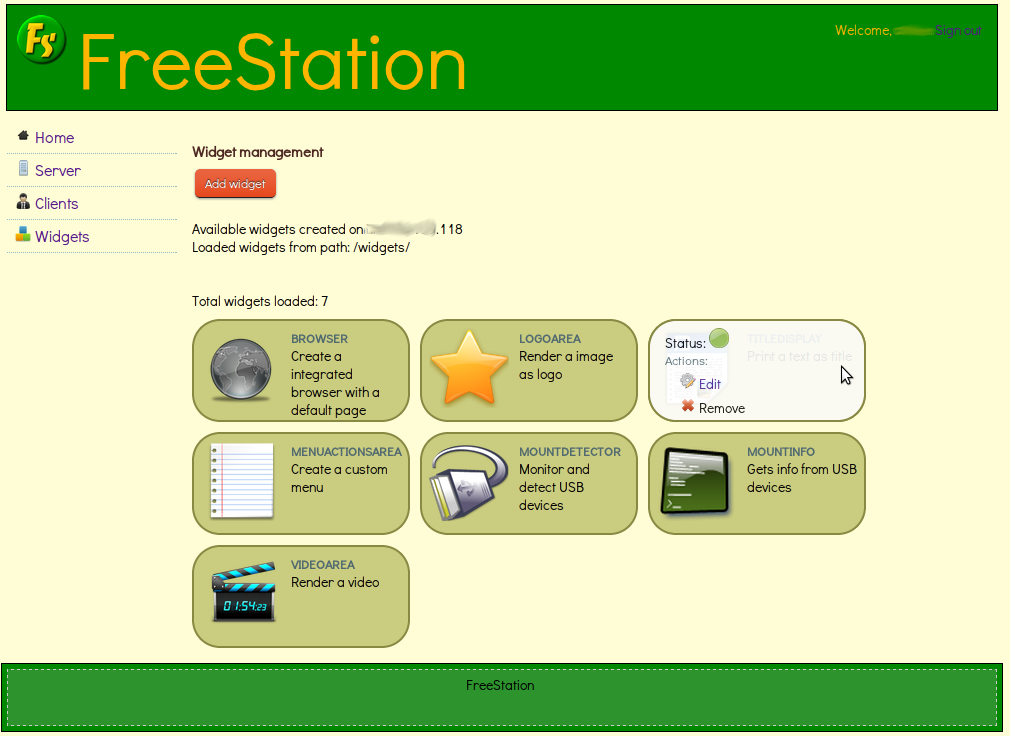
\includegraphics[scale=0.45]{src/img/freestation-server-widgets.png}
        \caption[FreeStation Server GUI - Listado de widgets iniciales] {FreeStation
        Server GUI - Listado de widgets iniciales}
    \end{center}
\end{figure}

\newpage

Los widgets cargados inicialmente en la configuración base son:

\begin{itemize}
    \item{*\textbf{MountDetector}: Detecta la presencia de unidades USB 
    (montaje/desmontaje) y recopila la información del nombre de la unidad, 
    espacio disponible y total.
    
    \begin{figure}[ht]
        \begin{center}
            
\includegraphics[height=32px]{src/img/widgets/mountdetector.png}
            \caption[Icono Widget MountDetector] {Icono Widget MountDetector}
        \end{center}
    \end{figure}}
    
    \item{*\textbf{MountInfo}: Configura una interfaz a partir de los datos de
    MountDetector con una barra de progreso para mostrar el espacio disponible/total.
    
    \begin{figure}[ht]
        \begin{center}
            
\includegraphics[height=32px]{src/img/widgets/mountinfo.png}
            \caption[Icono Widget MountInfo] {Icono Widget MountInfo}
        \end{center}
    \end{figure}}
    
    \item{*\textbf{VideoArea}: Carga un vídeo en reproducción continua y se
    activa en pantalla completa cuando FreeStation pasa a modo idle.
    
    \begin{figure}[ht]
        \begin{center}
            
\includegraphics[height=32px]{src/img/widgets/videoarea.png}
            \caption[Icono Widget VideoArea] {Icono Widget VideoArea}
        \end{center}
    \end{figure}}

    \item{\textbf{SliderArea}: Paneles informativos deslizantes con información
    para banners, transparencias, etc.}

    \item{*\textbf{GUI}: Inicializa la aplicación y lee los componentes
    habilitados para su carga, lanzándolos posteriormente.}
 
    \item{\textbf{CategoryArea}: Zona de información de listas verticales de
    categorías de información.}  
     
    \newpage
    
    \item{*\textbf{Browser}: habilita la navegación de una pagina web externa o
    documento html local.
    
    \begin{figure}[ht]
        \begin{center}
            
\includegraphics[height=32px]{src/img/widgets/browser.png}
            \caption[Icono Widget Browser] {Icono Widget Browser}
        \end{center}
    \end{figure}}
    
    \item{*\textbf{BrowserView}: renderiza templates según la vista (MVC: Modelo
    Vista Controlador) y trata con la lógica de la información proporcionada por
    el componente Browser.}


    \item{*\textbf{MenuActionsArea}: menú formado por flechas de
    anterior/siguiente/inicio para interactuar con las posibles zonas.
    
    \begin{figure}[ht]
        \begin{center}
            
\includegraphics[height=32px]{src/img/widgets/menuactionsarea.png}
            \caption[Icono MenuActionsArea] {Icono Widget MenuActionsArea}
        \end{center}
    \end{figure}}

    \item{*\textbf{LogoArea}: Carga un logo por defecto para la institución,
    universidad, escuela, oficina de turismo, ayuntamiento, etc.
    
    \begin{figure}[ht]
        \begin{center}
            
\includegraphics[height=32px]{src/img/widgets/logoarea.png}
            \caption[Icono LogoArea] {Icono Widget LogoArea}
        \end{center}
    \end{figure}}

    \item{\textbf{ClockArea}: Renderiza la hora actual.}

    \item{\textbf{ItemArea}: Muestra la información sobre algún elemento (puede
    ser software, documento, etc) con elementos como logo, descripción,
    dependencia, título.}     

    \item{*\textbf{TitleDisplay}: Carga un título central por defecto para la
    institución, universidad, escuela, oficina de turismo, ayuntamiento, etc.

    \begin{figure}[ht]
        \begin{center}
            
\includegraphics[height=32px]{src/img/widgets/titledisplay.png}
            \caption[Icono LogoArea] {Icono Widget TitleDisplay}
        \end{center}
    \end{figure}}

\end{itemize}

\newpage

Los widgets marcados con * han sido implementados completamente. El resto sólo
parcialmente o no son suficientemente estables en la versión presentada de este
documento.

\subsection{Composición de widgets y asociaciones}

Los widgets pueden componerse o asociarse.

Por ejemplo, se puede elegir distribuir y configurar un widget de almacenamiento
\acs{USB}\label{acro:USB} (USB Storage) y un widget de montaje (Mount Device) en
un cliente.

Esos widgets puede asociar operaciones para lista varios archivos de libros
sobre medicina. Cuando un usuario en un cliente POI, seleccione un libro y
escoja guardarlo en el USB, el widget de montaje detectará la presencia de un
USB conectado, e informará del espacio disponible gracias al widget de USB
Storage.

El widget de USB Storage se encargará de escribir los datos y esto
resultará en un usuario contento que ha obtenido la información rápidamente y
sin problemas en su dispositivo USB.

Pueden asociarse los widgets necesarios para un cliente, permitiendo
configuraciones personalizadas para cada cliente a través de parámetros
especializados en el widget. Por ejemplo, sólo permitir 5 elementos para guardar
en el widget de Mount Device).

\newpage

\begin{figure}[ht]
    \begin{center}
        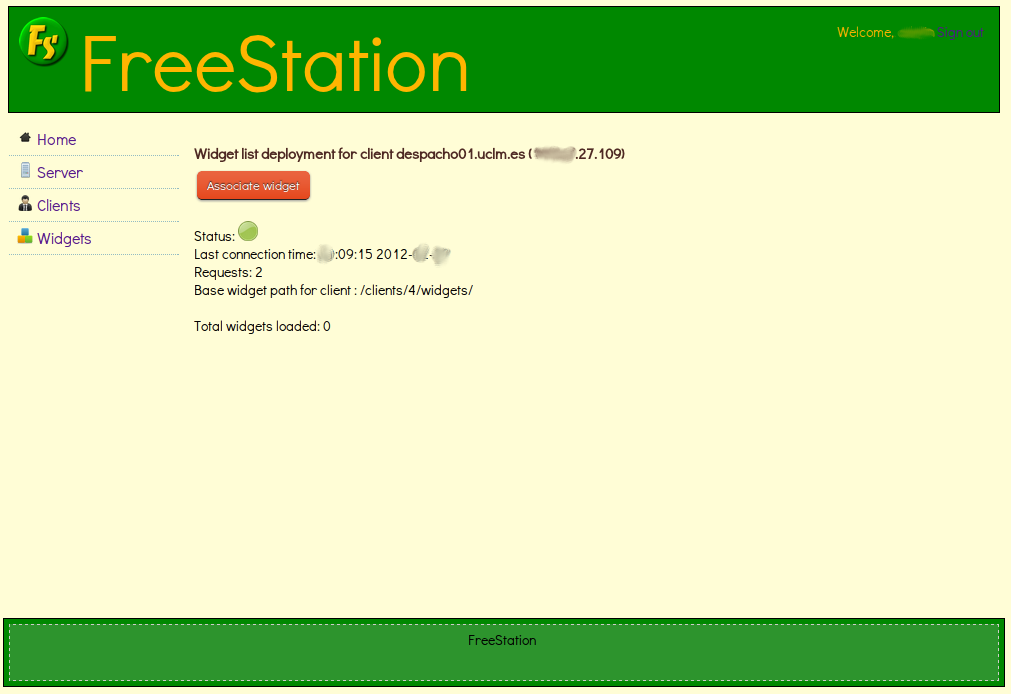
\includegraphics[scale=0.45]{src/img/freestation-server-associate-widget.png}
        \caption[FreeStation Server - Asociar un widget a un cliente] {FreeStation
        Server - Asociar un widget a un cliente}
        \label{fig:associateclient}
    \end{center}
\end{figure}

La figura ~\ref{fig:associateclient} muestra la asociación de un widget cliente 
en el servidor. Otro ejemplo, se puede elegir un widget de vídeo y habilitar que
se muestre un vídeo en un POI en modo inactivo.

Cuando el usuario toque la pantalla o interactúe de algún modo con el
POI, puede descargarse dicho widget y cargar un widget de navegador con
una página concreta.

De forma adicional, una institución podría elegir un simple logo y establecer el
widget para logos y que estuviera presente en toda pantalla mostrada usuario.

Cuando un cliente esta totalmente configurado, entonces puede ser desplegado
en el POI (como un ordenador de escritorio personalizado).

\newpage

\begin{figure}[ht]
    \begin{center}
        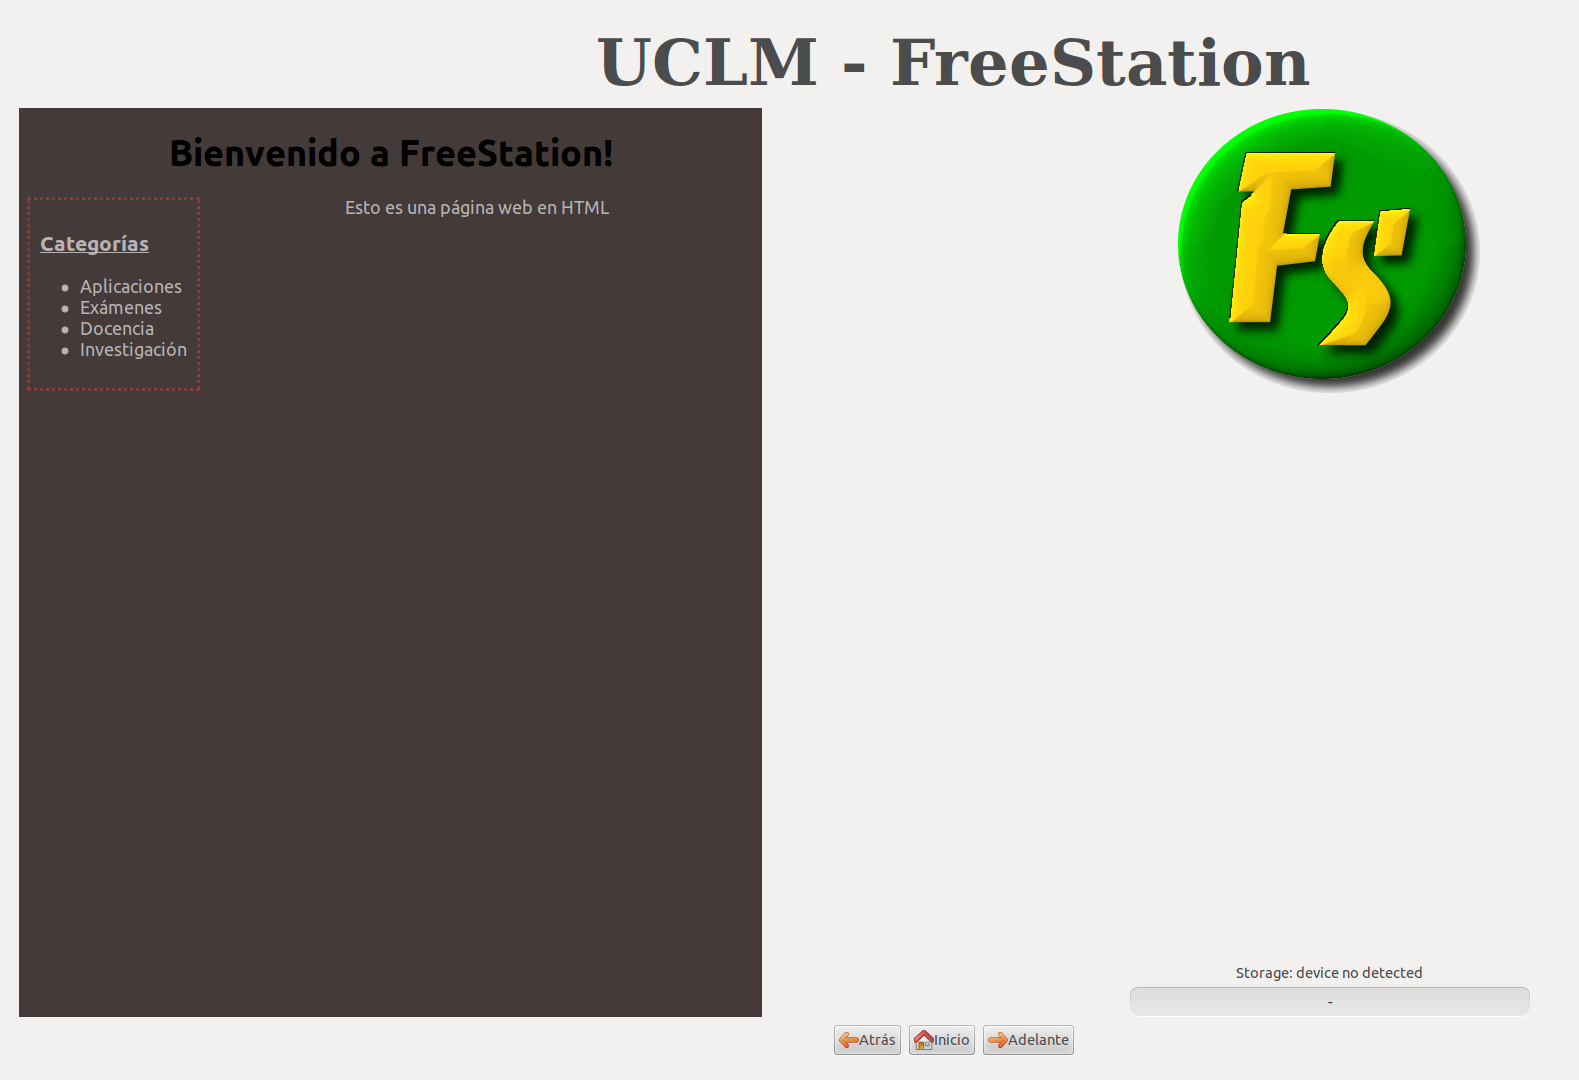
\includegraphics[width=460px]{src/img/welcome-client-widgets.png}
        \caption[Cliente FreeStation - Pantalla de bienvenida configurada] {Cliente FreeStation - Pantalla de bienvenida configurada}
        \label{fig:screendeploy}
    \end{center}
\end{figure}

En la figura ~\ref{fig:screendeploy} se puede apreciar un ejemplo de
pantalla de cliente desplegada. En esta pantalla desplegada en el cliente
existen varios widgets configurados.

Se ha configurado un widget Browser asociado a otro BrowserView para cargar una
pagina web HTML en un fichero local.

Por otro lado, se ha configurado un MenuActionsArea widget para mostrar los
botones de \emph{atrás/adelante/inicio} en la pantalla de bienvenida. A ello se
añaden un widget TitleDisplay para mostrar el título de bienvenida y un widget LogoArea
para cargar el logo de FreeStation.

Se presenta en el margen inferior izquierda un widget MountDetector asociado a
un widget MountInfo para mostrar la información actual. Este es sólo un ejemplo
posible de las muchas variaciones de configuraciones de widgets disponibles.
El usuario debe analizar los widgets necesarios para su aplicación y
configurarlos según su criterio.

\newpage

Por ejemplo para el widget BrowserView pueden configurarse el título de la web y
la web a cargar desde la configuración web en el servidor.

\begin{figure}[ht]
    \begin{center}
        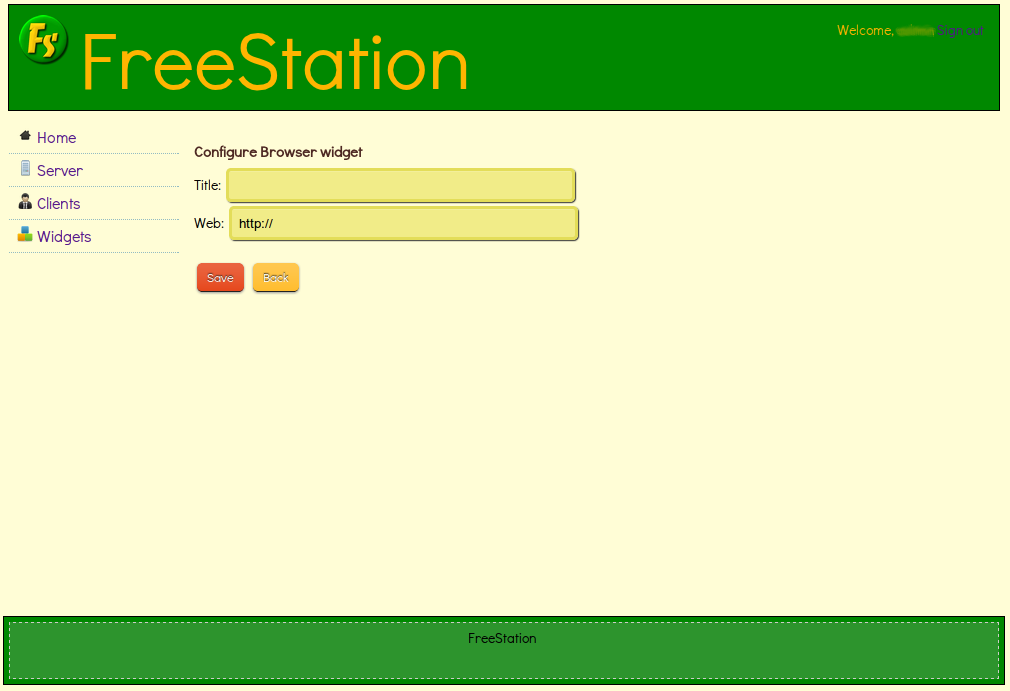
\includegraphics[scale=0.45]{src/img/freestation-server-configure-widget.png}
        \caption[FreeStation Server - Configurar un Widget para un cliente] {FreeStation
        Server - Configurar un Widget para un cliente}
        \label{fig:configurewidget}
    \end{center}
\end{figure}

Como muestra la figura ~\ref{fig:configurewidget} el usuario puede introducir
los datos específicos para su cliente POI.

\subsection{Fácil de escalar a nuevas necesidades}

No existe límite definiendo o usando nuevos widgets. En teoría el modelo de
widgets escala para cada tipo de necesidad personal para una organización,
institución, etc.

Con FreeStation algunos widgets básicos son ofrecidos por defecto, pero en el
futuro podría habilitarse un repositorio de widgets asociados, widgets de
empresas, widgets de asociados, etc y ofrecer un rico y amplio mercado para
desarrolladores que estén interesados en desarrollar widgets personalizados
para compañias, instituciones, hospitales, etc.

\newpage

\subsection{Arquitectura Watchdog}
\label{sec:watchdog}

Como se explico en el diagrama de flujo de la figura ~\ref{fig:flowclient} el
watchdog se apoya en un módulo que registra el estado de la aplicación 
principal (logger) para registrar toda actividad interrumpida o posibles 
fallos provocados en la aplicación.

Almacena los identificadores de procesos relativos a las instancias monitorizadas y capta señales
de interrupción de la aplicación como SIGTERM o excepciones no capturadas en niveles superiores.

En el momento de la implementación del lanzador se valoró usar el módulo 
multiprocessing nativo de Python, pero el
rendimiento y legibilidad en el código empeoraban considerablemente el 
watchdog resultando poco
efectivo y tolerante a fallos.

En una implementación posterior del lanzador, se implemento como un hilo 
(Thread) para aprovechar las ventajas
del COW (Copy-On-Write) en GNU/Linux, además de separar la interfaz y 
lógica de negocio de la aplicación
en diferentes procesos.

El watchdog también identifica cada hilo con un nombre único compuesto por:

$<CLIENTE>-<TIMESTAMP>$

Siendo CLIENTE, el nombre del cliente POI, por defecto «FreeStation» y 
TIMESTAMP el instante de tiempo en epoch
unix que fue lanzado. De esta forma, a través del módulo logger puede 
identificarse el hilo lanzado que tuvo
un fallo y analizar el mismo a través de depuración de la aplicación.

Para propósitos de pruebas (test) el módulo incluye un parámetro temporizador 
de tiempo con vida «alive time» desactivado
por defecto para que sea posible monitorizar solo por un intervalo de tiempo 
y finalizar el watchdog.

Asimismo se incluye otro parámetro/flag para test que permite ejecutar el 
watchdog sin la presencia de interfaz gráfica
para ejecutar test unitarios de forma más rápida y sin intervención manual.

\newpage

El tiempo de monitorización por defecto esta establecido a 1 segundo. Este 
valor resulta óptimo ya que en caso de
producirse fallo de la aplicación y se lance de nuevo, el usuario no tendrá 
capacidad de reacción para intervenir en el fallo
e instantáneamente tendrá de nuevo usable la aplicación.

\subsection{Arquitectura del lanzador}

El lanzador tras ser invocado por el watchdog inicialmente es cargado como una
subclase Thread del módulo python que recibe el nombre de FreeStationApp.

En su inicialización, se activa el módulo logger guardando en ficheros de
registro cada evento de información importante.

Se hacen las comprobaciones previas de bibliotecas necesarias como GTK 3.0,
limitación por lógica de una sola instancia de aplicación (ya que el cliente
sólo podrá ser ejecutado una vez por POI).

Se guarda el PID del proceso padre, que coincidirá con el proceso Watchdog, al
igual que también se guarda el PID del propio thread y el nombre asignado al
thread que como se comentó en la sección \ref{sec:watchdog} recibe el nombre
$<CLIENTE>-<TIMESTAMP>$.

Se comprobará si se ha establecido un tiempo de vida para el hilo (para
propósitos de pruebas unitarias) y si se ha habilitado el flag de GUI para
iniciarlo (deshabilitado en caso de pruebas unitarias).

Si se cumplen las condiciones, se iniciará el módulo GUI que interactuará con el
bucle principal de GTK.

Si la aplicación finaliza por algún motivo inesperado, el lanzador tratará de
escribir los datos en el registro y el watchdog en su comprobación llamará de
nuevo al lanzador para que reinicie la aplicación.

\newpage

\subsection{Manejo de excepciones}
\label{sec:exceptions}
Las excepciones en la programación de FreeStation están presentes en el flujo
del programa. La gestión de excepciones permite un mayor control del mismo e
interpretar de forma más correcta cualquier posible error para su depuración. 

La excepción base para cliente y backend basado en python esta implementada en
la clase \emph{FSBaseException}.

Es la encargada de establecer los métodos comunes y establecer un patrón de
especialización (subclassing) para el resto de excepciones a partir de la clase
nativa Exception de python. Se establece también el formato de errores de
impresión para el resto de excepciones. Por tanto, se consolida el mismo
concepto base de excepciones y comportamiento para todas las excepciones
derivadas en la aplicación.

De esta forma excepciones de más alto nivel pueden utilizarse a partir de dicha
implementación base. Un ejemplo son las excepciones siguientes:

\begin{itemize}
  \item ClientStatusDisabled: lanzada cuando un cliente FreeStation accede al
  servidor con un estado marcado como desabilitado.
  \item NoAuthorized: lanzada cuando un cliente FreeStation accede sin
  autorización al servidor.
\end{itemize} 

\begin{figure}[ht]
    \begin{center}
        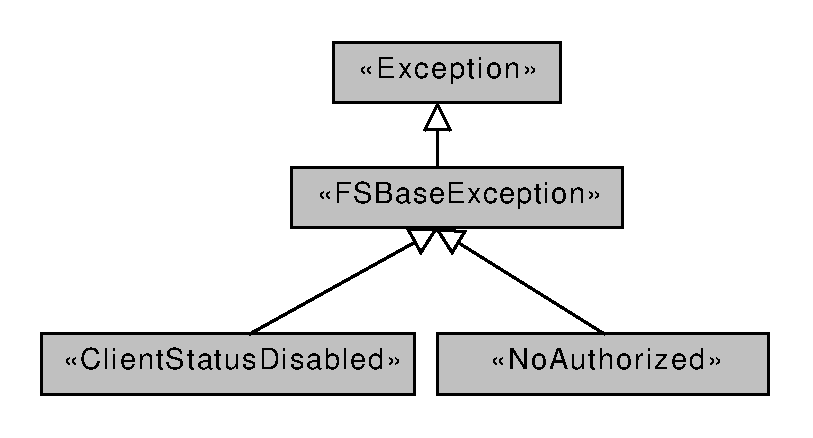
\includegraphics[width=300px]{src/img/diagrams/freestation-class-diagram-exceptions.pdf}
        \caption[Diagrama de clases para excepciones]
          {Diagrama de clases para excepciones}
          \label{fig:classexceptions}
    \end{center}
\end{figure}

\newpage

El diagrama de clases de la figura ~\ref{fig:classexceptions} representa la
estructura de clases para dichas excepciones.

Estas excepciones proveen los medios para separar los detalles en el momento
de producirse un comportamiento no esperado y fuera de la lógica principal del
programa.

Cada cliente FreeStation debe conocer todas las excepciones posibles derivadas
en llamadas al servidor. Con ese objetivo es posible un total control de
excepciones (para consolidar un sistema probado como se explico en la sección
~\ref{sec:poiproduccion}). Los casos no contemplados pueden tratarse
genéricamente y establecer una acción de recuperación o 
vuelta al estado original.

\subsection{Test unitarios}

El conjunto de pruebas permiten evaluar el correcto funcionamiento del sistema y
cómo se adapta a las especificaciones descritas en la definición de requisitos.

Durante el desarrollo de este proyecto de fin de carrera se han realizado varios
tipos de test. Pruebas de características con ejemplos simples de funcionamiento
y pruebas unitarias.

Las pruebas de características se encuentran en el directorio tests de la
carpeta raíz del proyecto. En el caso del cliente se realizan pruebas como
funcionamiento de vídeo en GTK2 y GTK3, ejemplo de vídeo mínimo, ejemplo de
carga para Webkit, temporizador, diferentes pruebas de características de
Gstreamer (factoría de elementos multimedia, reloj multimedia, sincronización
de vídeo, etc)

Por otro lado, los test unitarios se encuentran en directorio
freestation/test/unit los test unitarios permiten el desarrollo continuo de una
aplicación asegurando su calidad en cada pequeña modificación. Todos los 
test unitarios comparten la especialización (subclassing) de la clase 
BaseUnitTest. 

A partir de la clase TestCase del módulo unittest establece los métodos comunes
inicializadores (setUp) y finalizadores (tearDown) del resto de test unitarios.

\newpage

\section{\uppercase{Patrones de ingeniería del software utilizados}}
\label{sec:patrones}
Los patrones software\cite{GHe06} principalmente usados en este proyecto de fin
de carrera han sido:

\begin{itemize}
  \item \textbf{Singleton}: su propósito es asegurar que sólo exista una
  instancia de una clase. Es un patrón creacional que garantiza la existencia de un mecanismo de
  acceso global a dicha instancia. Se ha utilizado en clases de \emph{Frontend}
  del servidor como \emph{CMS}, \emph{Session}, \emph{Error} y
  \emph{ClassHash}.
  \item \textbf{Factory o Fábrica}: es un patrón creacional que centraliza en
  una clase constructora la creación de objetos de un subtipo de un tipo determinado, 
  ocultando al usuario la casuística para elegir el subtipo que crear. Se ha
  utilizado en clases relacionadas con CouchDB como \emph{HubFactory} y la
  creación de widgets.
  \item \textbf{Mosca o peso ligero(Flyweight)}: es un patrón estructural que
  reduce la redundancia cuando gran cantidad de objetos que poseen idéntica información.
  Se ha utilizado en la creación de widgets para una carga más ligera.
  \item \textbf{Facade (Fachada)}: es un patrón estructural que provee de una
  interfaz unificada simple para acceder a una interfaz o grupo de interfaces de un 
  subsistema. Es utilizado en las clases de \emph{Frontend} del servidor para
  la creación de la \emph{Api} y su administración con la clase
  \emph{ApiManager}
  \item \textbf{Proxy}: es un patrón estructural que mantiene un representante
  de un objeto.
  Se ha utilizado en la conexión de Zero C ICE para comunicación con el cliente
  y servidor.
  \item \textbf{Adapter (Adaptador)}: es un patrón estructural que adapta una
  interfaz para que pueda ser utilizada por una clase que de otro modo no podría utilizarla.
  Se ha utilizado en la conexión de Zero C ICE para comunicación con el cliente
  y servidor.
\end{itemize}

Como patrón de diseño se ha utilizado \acs{MVC}\label{acro:MVC} para el
\emph{Frontend} del servidor como se explico en la sección
~\ref{sec:interfazderivada}.

\newpage

\subsection{GUI: Clase de interfaz gráfica}
\label{sec:widgetloader}
Esta clase posee toda la lógica de control de la interfaz de usuario. Es la
encargada de generar dinámicamente la interfaz a través de los datos
proporcionados y configurados en el cliente FreeStation.

Proporcionado los interfaces genéricos lleva a cabo un cargado inicial de cada
componente. Por un lado, es capaz de integrar en un thread, que servirá para
establecer un cliente del tipo \emph{FreeStationApp} y capturar
la recepción y envío de mensajes.

La clase \emph{FreeStationApp} inicializa en el thread. En el mismo se
establecen los eventos para el sistema de objetos de GLib
(\acs{GObject}\label{acro:GObject}) y \acs{GDK}\label{acro:GDK} necesarios para
los bindings de python y posteriores widgets.

Es importante recalcar que en el thread es necesario inicializar como thread
independiente GDK a través de la función $Gdk.threads\_init()$ y establecer las
condiciones de guarda de entrada y salida con $Gdk.threads\_enter()$ y
$Gdk.threads\_leave()$ respectivamente. Dentro de estas condiciones es posible
inicializar el principal bucle de eventos de GTK con $Gtk.main()$.

En ese momento la clase \emph{GUI} es cargada como un meta widget general
desde $widgets.GUI$. La clase \emph{GUI} es una subclase o
especialización del elemento Window de GTK. Aplica los atributos de una 
ventana principal a tamaño completo por defecto.

Establece asociaciones con diferentes atajos de teclado. Dispone de los atajos
de teclado pulsando la tecla f minúscula para cambiar el modo de pantalla 
completa (a modo depuración, debe ser deshabilitado en
producción), al igual que la tecla q, para simulara el cerrado de la aplicación
y que el Watchdog lo detecte reiniciando la aplicación.

Esta clase se encarga principalmente de cargar la configuración XML
proporcionada por el cliente a través de la clase WidgetLoader. A través de la
ejecución del método privado $\_\_load_widgets$ se realizará una petición de
datos en la que se invoca y delega la tarea a la clase \emph{WidgetLoader}.

\newpage
Una vez la configuración es proporcionada por WidgetLoader, se realiza una carga
dinámica de la clases de forma metaprogramada.

\begin{lstlisting}[language={Python}, label={lst:wigdetsloaddinamic},
texcl=false, caption={Carga dinámica de clases - Metaprogramación}]
self.widgets = WidgetLoader().get_widgets()

for (name, properties) in self.widgets:

    widget_error = False
    
    mod = __import__('freestation.widgets', fromlist = [str(name)])
    
    try:
        mod_class = getattr(mod, name)
    except AttributeError, e:
        print 'Error: could not load the widget ' + name
        widget_error = True
      
    if not widget_error:  
        klass = getattr(mod_class, name)
        
        temporal_object = klass()
        
        temporal_attribute = temporal_object.__class__.__name__
           
        # Create lowercase with underscore
        # attribute class from name widget
        name_attribute = ''
        i = 0
        for letter in temporal_attribute:
            if letter.isupper():
                if i == 0:
                    letter = letter.lower()
                else:
                    letter = '_' + letter.lower()
                
            name_attribute += str(letter)
            i += 1
           
        # Create attribute on class with metadinamic class created
        setattr(self, name_attribute + '_widget', temporal_object)
\end{lstlisting}

En el listado de código ~\ref{lst:wigdetsloaddinamic} se expone la
metaprogramación implicada para la carga de widgets. Mediante el módulo
importlib (función $\_\_import\_\_$) de python se cargan todos los widgets
configurados en la lista XML recibida. Esta lista XML recibe un formato 
específico que es procesado y devuelto en formato de listas y 
tuplas de python, conteniendo el nombre del widget y las
propiedades asociadas al mismo. En el proceso de carga de datos se realizan
algunas adaptaciones de los nombres de clase nombrados en formato 
camelCase\footnote{camelCase: \url{http://es.wikipedia.org/wiki/CamelCase}
\label{ftn:camelCase}}, a formato con guiones bajos para python y sus módulos.

Los widgets son cargados dinámicamente en tiempo de ejecución desde los módulos
existentes en freestation.widgets. Se realiza una comprobación si se intenta
cargar un módulo de widget por XML que el cliente no haya recibido del servidor.

En caso de no existir errores en la carga de widgets, se carga dinámicamente la
clase del widget desde el módulo de widget y se invoca en tiempo de ejecución
para crear un objeto. Para guardar la referencia, se crea un atributo a la clase
GUI en tiempo de ejecución. Posteriormente la clase invocará el empaquetado y
disposición del los widgets cargados a través de dichos atributos creados 
dinámicamente.

\begin{figure}[ht]
    \begin{center}
        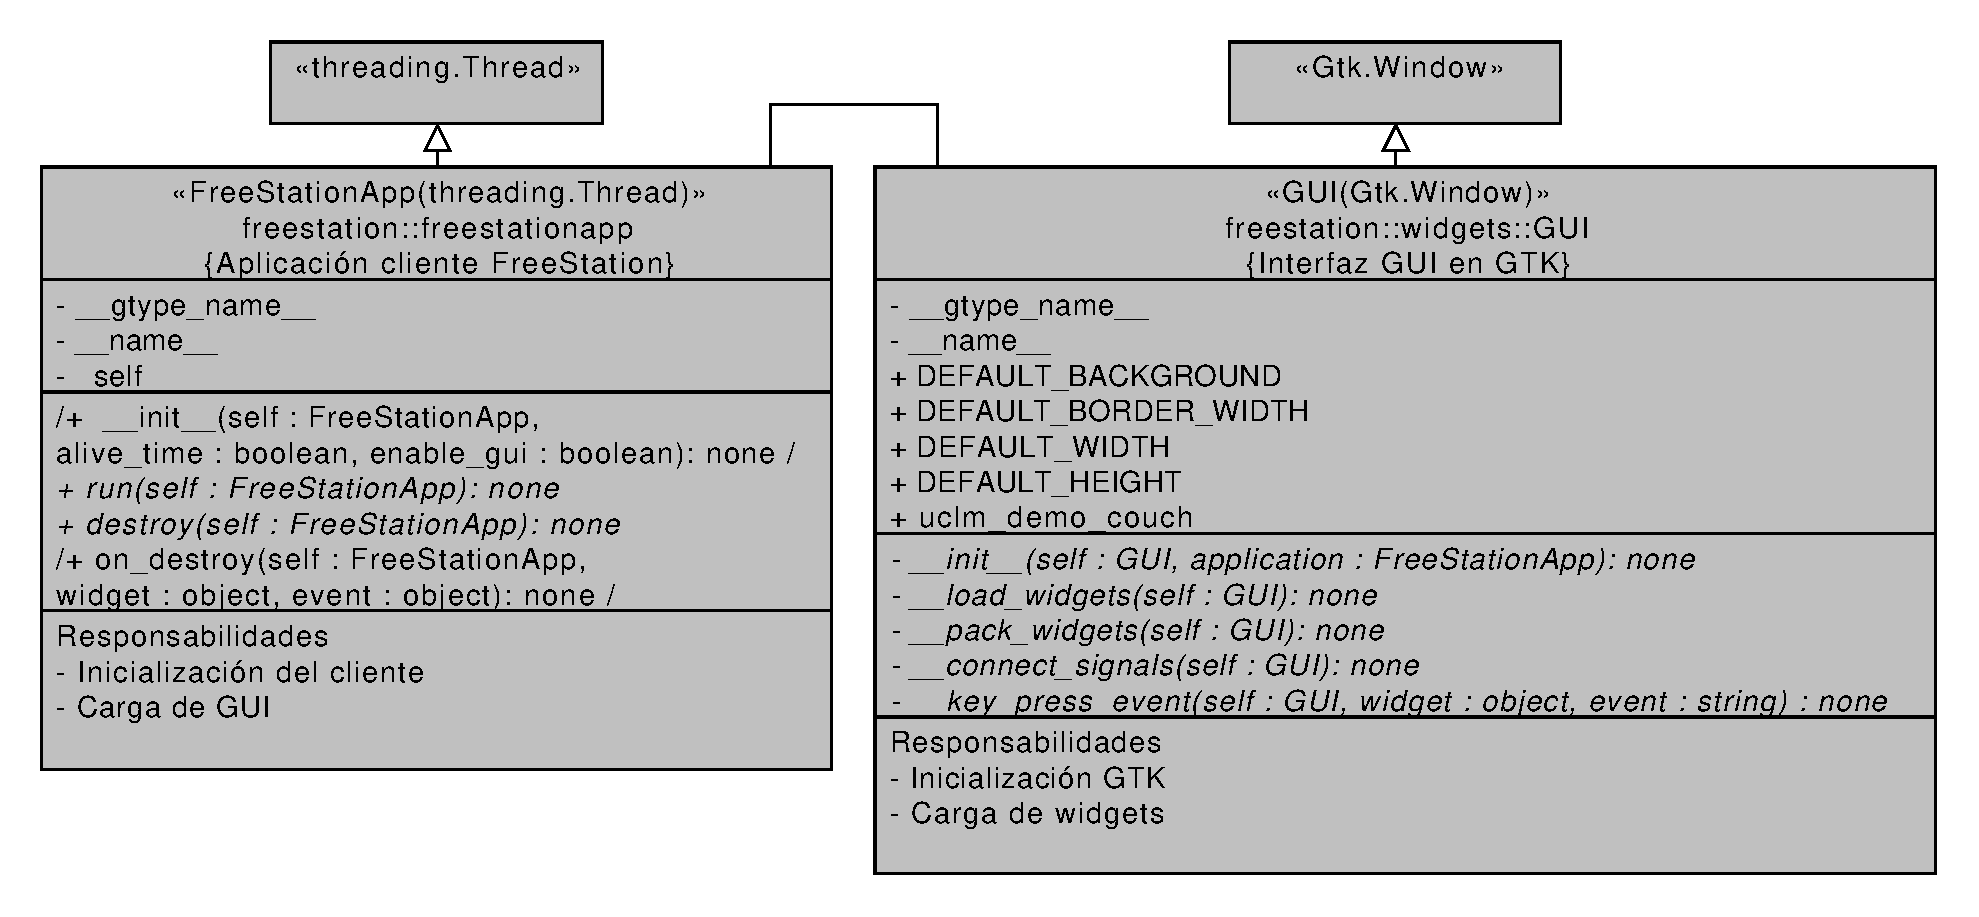
\includegraphics[width=425px]{src/img/diagrams/freestation-class-diagram-freestationapp.pdf}
        \caption[Diagrama de clases FreeStationApp y GUI]
          {Diagrama de clases FreeStationApp y GUI}
        \label{fig:classgui}
    \end{center}
\end{figure}

En el diagrama de clases de la figura ~\ref{fig:classgui} se detalla el diseño y
estructura de las clases \emph{FreeStationApp} y \emph{GUI}.

\newpage

\subsection{WidgetLoader: cargador dinámico de widgets}

Es la clase encargada de procesar el archivo widgets.xml recibido del servidor.
El formato de widgets.xml sigue un formato especial.
\begin{lstlisting}[language={XML}, texcl=false, ,
label={lst:wigdetsxml}, caption=Ejemplo de configuración XML para
archivo widgets.xml] <?xml version="1.0" encoding="UTF-8"?>

<interface>

    <widget>
        <name>TitleDisplay</name>
        <properties>
            <position type="relative" child="0" pack="None|Start|End">MainWindow</position>
            <homogeneous>1</homogeneous>
            <spacing>5</spacing>
            <width>200</width>
            <height>300</height>
            <data>UCLM - FreeStation</data>
        </properties>
    </widget>
    
    <widget>
        <name>BrowserView</name>
        <properties>
            <position type="absolute"></position>
            <width>200</width>
            <height>300</height>
        </properties>
    </widget>
    
    <widget>
        <name>MountInfo</name>
        <properties>
            <position type="absolute"></position>
            <width>200</width>
            <height>300</height>
        </properties>
    </widget>
    
</interface>
\end{lstlisting}

\newpage

En el ejemplo ~\ref{lst:wigdetsxml} puede observarse que todo widget
necesariamente debe ir etiquetado bajo la marca de entidad XML ``interface''.
Posteriormente una serie de conjuntos ilimitados de widgets pueden ser listados
mediante la entidad ``widget''. Toda entidad widget debe contener al menos una
entidad ``name'' y otra entidad ``properties'' en su interior.

Las propiedades definen un conjunto de características según el widget. Estas
características son dependientes de la implementación en python que se realice.
Sólo serán reconocidas las características que la implementación en python del
widget reconozca.

Por ejemplo para un widget pueden definirse posiciones relativas o absolutas a
otros widgets, pero esta funcionalidad no esta completamente implementada.
De igual forma pueden establecerse el ancho y alto del widget, espacio entre
widgets, distribución homogénea y datos de preconfiguración cargados.

Todo evento de información que suceda es también guardado mediante la clase
Logger en el registro general de eventos.

La clase WidgetLoader además realiza comprobación de integridad del fichero
widgets.xml. Si por ejemplo existen errores al definir las entidades interface,
widgets, etc.

Si algún error es detectado, como se comento en la sección
~\ref{sec:exceptions} se lanza una excepción a la clase superior, en este caso
GUI, para que trate adecuadamente el widget o conjunto de widgets que no 
pudieron ser cargados.

En particular existen excepciones de alto nivel que son lanzadas si se
detecta algún problema y con las que el cliente FreeStation debe capturarse.

Todas las excepciones lanzadas son especializaciones de la clase
\emph{FSBaseException}.

\newpage
Las principales excepciones son:
\begin{itemize}
    \item \textbf{WidgetXMLFileNotFound}: lanzada cuando el archivo widgets.xml no
    esta presente o no tiene permisos de lectura.
    \item \textbf{WidgetXMLBadFormed}: lanzada cuando el archivo widgets.xml no
    contiene un formato XML válido o es imposible continuar el análisis del mismo.
\end{itemize}

La clase WidgetLoader basa su implementación en el módulo
minidom\footnote{Módulo minidom python:\\
\url{http://docs.python.org/library/xml.dom.minidom.html}
\label{ftn:minidom}} de python que
le permite diferenciar entre nodos, datos, entidades XML. 

Inicialmente se intenta leer y cargar el archivo XML widgets.xml desde la 
función $\_read\_data$ y $\_load\_xml$. Sino se encuentra un éxito se
lanzará la excepción \emph{WidgetXMLFileNotFound}, de lo contrario se 
intentará analizar el modelo de documento de objetos (DOM).

Si se dispone de un DOM, se intentarán validar etiquetas como nodos por 
ejemplo como las etiquetas interface, widgets, etc.
En caso fallido se lanzará la excepción \emph{WidgetXMLBadFormed} y se 
intentara seguir leyendo
el archivo para análisis de otros posibles widgets.

\begin{lstlisting}[language={XML}, texcl=false, ,
label={lst:xmlnodes}, caption=Tipos de nodos XML]
ELEMENT_NODE                = 1
ATTRIBUTE_NODE              = 2
TEXT_NODE                   = 3
CDATA_SECTION_NODE          = 4
ENTITY_REFERENCE_NODE       = 5
ENTITY_NODE                 = 6
PROCESSING_INSTRUCTION_NODE = 7
COMMENT_NODE                = 8
DOCUMENT_NODE               = 9
DOCUMENT_TYPE_NODE          = 10
DOCUMENT_FRAGMENT_NODE      = 11
NOTATION_NODE               = 12
\end{lstlisting}

\newpage

El listado ~\ref{lst:xmlnodes} ofrece todos los tipos de nodos XML disponibles
con sus valores designados y que son analizados en el proceso. En particular los 
elementos de información útil serán $ELEMENT\_NODE$ que son filtrados
a partir de la función $\_filter\_element\_nodes$. 

En ellos, se encuentra la información del valor del nodo, que será almacenado en
formato de tuplas python y devuelto como resultado a capas superiores.

\begin{figure}[ht]
    \begin{center}
        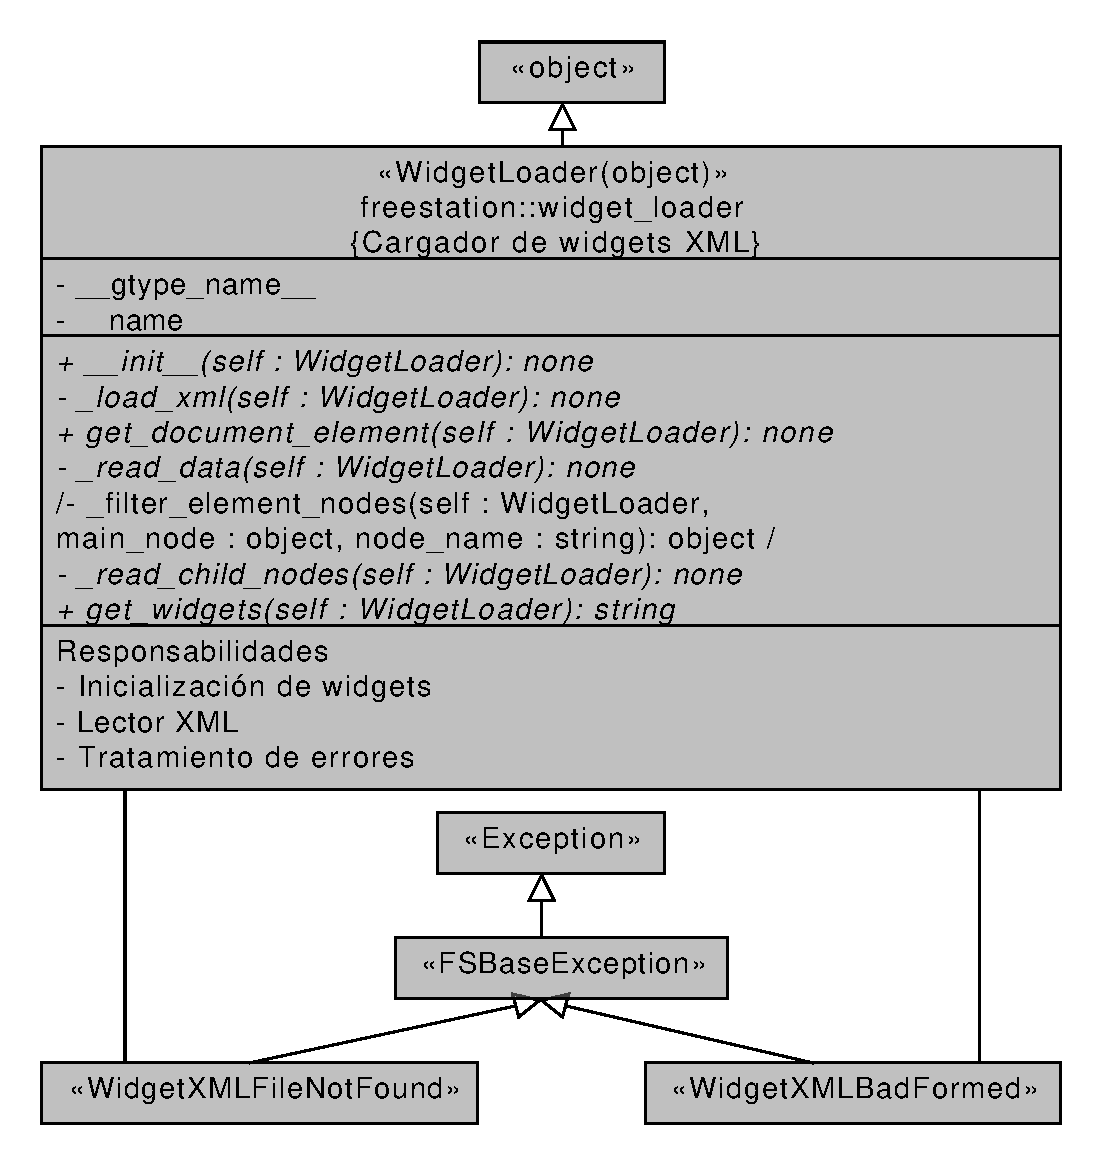
\includegraphics[width=425px]{src/img/diagrams/freestation-class-diagram-widgetloader.pdf}
        \caption[Diagrama de clases FreeStationApp y GUI]
          {Diagrama de clases WidgetLoader}
        \label{fig:widgetloader}
    \end{center}
\end{figure}

El diagrama de clases ~\ref{fig:widgetloader} ilustra la clase WidgetLoader y
sus excepciones.

\newpage

\subsubsection{Backend}
\label{sec:backendice}

El \emph{Backend} esta desarrollado como un módulo independiente. Dicho módulo
esta basado en una aplicación Ice llamada \emph{FreeStationServer}. Por otro lado, el
\emph{Backend} es inicializado mediante el servidor web \emph{Frontend}
en PHP.

\textbf{Backend ZeroC ICE}

En esta sección se describirá el subsistema de \emph{Backend} para lado servidor
basado en ZeroC ICE, su cometido, su funcionalidad y su implementación.

ZeroC ICE es el middleware por excelencia para sistemas distribuidos como se
explico en la sección ~\ref{sec:ZeroICE}.

La potencia de invocación de objetos remotos como si fueran objetos locales hace
posible el funcionamiento de la clase \emph{FreeStationServer}. La aplicación
internamente realiza una enmascaración mediante un proxy para la parte del
cliente.

El desarrollo distribuido permite un gran potencial. Una vez es inicializado
por parte del \emph{Frontend} se invoca una instancia de
\emph{FreeStationServer}, que se basa en una especialización de la clase \emph{Ice.Application}.

Dicha clase, necesita de una configuración inicial de propiedades que por 
defecto son almacenadas en la clase controladora.

Como se explicó en la sección ~\ref{sec:generacionint} FreeStation usa un MVC y
una capa de datos basada en XML. El servidor necesita un esqueleto que
traduzca los eventos entre la comunicación con el cliente. La comunicación no
deja de ser una comunicación que sigue protocolos de red estándar como TCP o UDP.

Por este motivo, FreeStation utiliza esta estructura internamente para
representar las configuraciones. La clase ICE llamada
\emph{Ice.InitializationData} permite establecer propiedades de configuración.

A través del método $init\_properties$ las configuraciones se establecen en
tiempo de ejecución desactivando la posibilidad de carga externa de 
configuraciones por archivos de configuración de
ICE. La directiva ICE utilizada es $Ice.Config$.

Con propósitos de identificación de la aplicación se establece un nombre del
proceso ICE con la directiva de configuración $Ice.ProgramName$

Para evitar problemas de limites de memoria ($Ice::MemoryLimitException$) se
establece un tamaño máximo de mensaje de 10 MB en lugar de 1 MB establecido por
defecto con la directiva $Ice.MessageSizeMax$.

Si esta activo el modo depuración de FreeStationServer (activado con el flag
$DEBUG$) se imprimirá el PID del proceso con $Ice.PrintProcessId$

Por otro lado se establecen los ficheros de salida estándar y error con
$Ice.StdErr$ e $Ice.StdOut$ y el modo NOHUP para el proceso con $Ice.Nohup$.
Las trazas de la aplicación están activadas con el fin de mejorar la información
mostrada en el \emph{Frontend} para ello se utiliza la directiva
$Ice.PrintStackTraces$ y un modo excesivamente de depuración si trazas si esta
activo el flag $DEBUG$. De la misma forma se activan otras configuraciones con
el fin de mejorar el rendimiento de la aplicación.

Una vez se ha establecido toda la configuración necesaria, se procede a la carga
de ficheros slice .ice.

La carga de la interfaz es realizada por el método $load\_ice\_interface$. Este
buscará una especificación de archivo slice en $ice/fs.ice$ y cargará el slice
en tiempo de ejecución con $Ice.loadSlice$. Para ello debe estar previamente
generado. Si se detecta que no ha sido generado, se procederá a generarlo con un
comando del tipo:

\begin{lstlisting}[language={bash}, texcl=false, caption={}]
[["cpp:include:list"]]
slice2py --underscore --output-dir . ice/fs.ice
\end{lstlisting}

Esto generará un directorio FS (módulo) con el slice generado como código
Python.

\newpage

\textbf{Especificación slice para ICE}

Un archivo de especificación Slice es un lenguaje de definición de
interfaces\footnote{The Slice Language:\\
\url{http://doc.zeroc.com/display/Ice/The+Slice+Language}
\label{ftn:slicelang}} usado por ICE. Es un mecanismo de abstracción para
separar las interfaces de objetos de sus implementaciones. Define un contrato entre
servidor-cliente para una aplicación, incluyendo las interfaces, 
operaciones, parámetros, tipos de datos y excepciones.

La descripción es independiente del lenguaje de implementación. La sintaxis de
Slice tiene un gran parecido con la sintaxis de C++ o Java por lo que es 
fácilmente reconocible.

A dichos contratos se les denomina en inglés ``push model'' o ``pull model''
dependiendo del lado que lo emita (emisor o receptor). En ocasiones un
mismo modelo puede ser push/pull de ambos tipos a la vez.

Las definiciones del Slice se compilan en particular para el lenguaje en el
que son implementadas por un compilador.
Esto permite al compilador traducir definiciones escritas en un lenguaje
independiente a un lenguaje especifico de definiciones de tipos y APIs. Es por
tanto un lenguaje puramente declarativo.

\begin{figure}[ht]
    \begin{center}
        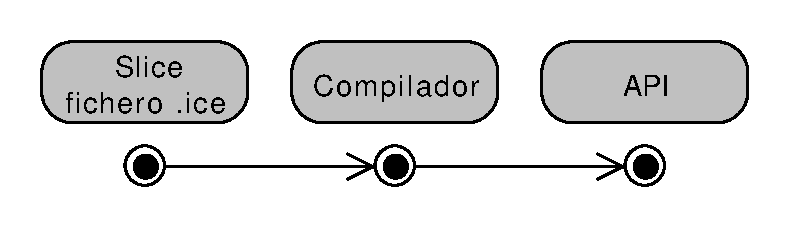
\includegraphics[width=425px]{src/img/diagrams/freestation-states-slice-diagram.pdf}
        \caption[Diagrama de estados compilación Slice]
          {Diagrama de estados compilación Slice]}
        \label{fig:stateslice}
    \end{center}
\end{figure}

Su principal enfoque esta en las interfaces de objetos y las operaciones que
definen. Los objetos también pueden ofrecer persistencia de objetos a través de
la definición de tipos de datos. Esto es posible gracias al intercambio de datos
entre cliente y servidor, de esta forma se evitan intercambios de datos
arbitrarios y sin estructurar.

\newpage

El módulo FS es autogenerado a partir del archivo slice fs.ice que actúa de
igual forma como contrato modelo push/pull para cliente y servidor.
El archivo de especificación es el siguiente:

\begin{lstlisting}[language={bash}, texcl=false, caption={Especificación slice
para ICE}] [["cpp:include:list"]]

module FS 
{
   sequence<byte> File;
   
   sequence<byte> FileBlock;
   
   interface Api 
   {
     void getWidgets();
     string getXMLWidgets();
     void version(out string sout);
     int getFileSize(string path);
     File getFile(string path);
     FileBlock getFileChunk(string path, int pos, int size);
     void isAuthorized(out bool sout);
     int getClientId();
   };
   
   interface Widget 
   {
     void getName();
   };
   
   exception GenericError 
   {
     string reason;
   };
   
   exception NoAuthorized extends GenericError{};
};
\end{lstlisting}

En el se define un módulo FS, con varias interfaces, tipos de datos y
excepciones.

Los tipos de datos $File$ y $FileBlock$ son definidos como secuencias de bytes y
serán utilizados para la transferencias de ficheros de las interfaces. Las
principales interfaces definidas son $Api$ y $Widget$. La interfaz $Api$ define
unos métodos para la administración y comprobación de privilegios al conectar al
misma con $isAuthorized$. Métodos como $getClientId$, $getWidgets$, etc son
métodos usados en la Api para comunicación entre cliente y servidor.

\newpage

\textbf{Creación del comunicador}

Una vez el servidor es configurado, creado el fichero slice, se ejecuta
con el método $start$ y este llama al $main$ de la clase padre
\emph{Ice.Application}. Tras ello, el método invocado es $run$ que es sobreescrito en
la clase hija \emph{FreeStationServer}.

En ese momento se crea un comunicador siguiendo el modelo de hilos de Zero C
ICE\footnote{The Ice Threading Model:\\
\url{http://doc.zeroc.com/display/Ice/The+Ice+Threading+Model}
\label{ftn:icethread}}. El comunicador es el encargado de crear un contexto
implícito y gestionar los eventos de la clase \emph{Ice::Router}. Este contexto
será accesible posteriormente y servirá para guardar datos de utilidad como
número de peticiones servidas para cada cliente. Las propiedades del comunicador
podrán visualizarse con el método $show\_communicator\_properties$.

\textbf{Creación del adaptador y puntos finales de conexión}

Cuando se ha establecido la comunicación, es necesario crear un objeto
adaptador. Su principal funcionalidad será mapear los objetos ICE a los
sirvientes (servants) que comparten los hilos creados por el comunicador.
También es posible configurarlo como individual para disponer de una reserva de
hilos privada. El método $create\_adapter$ creará el adaptador y tratará con
cualquier error que pueda suceder. 

Los puntos finales de conexión son gestionados con la clase \emph{Ice.Endpoint}.
FreeStation usa por defecto el protocolo UDP en el puerto 10000 ya que no
necesita confirmación (ACK) de los mensajes, ya que ICE asegura la recepción. De esta
forma se consigue una mayor tasa de transferencia en el envío de archivos y
conexiones. La información sobre puntos finales de conexión puede visualizarse
con el método $show\_endpoints\_info$. En caso de existir varias IPs en la
máquina servidor o conexión a varios puertos, la conexión aumentará de
rendimiento al disponer de mayores puntos de conexión.

\textbf{Creación del sirviente}

Una vez creado el adaptador se creará una instancia de sirviente. Un sirviente
mantiene todos los objetos de ICE en memoria. Los sirvientes están optimizados
para no almacenar demasiados estados en memoria y evitar el exceso de recursos
escalando apropiadamente. El método $create\_servant$ es el encargado de crear
el sirviente.

\newpage

\textbf{Módulo FS.Api}

Este módulo es autogenerado en código python como resultado de la compilación
del slice. Mapea mediante clases temporales las interfaces con
$Ice.createTempClass()$. Establece el proxy para comunicación entre
cliente y servidor mediante \emph{Ice.Object} y \emph{Ice.ObjectPrx}. Las
operaciones de las interfaces son mapeadas en la autogeneración con a través de
$IcePy.Operation$ indicando los parámetros de la operación y el modo de
operación (normal o idempotente). Las excepciones sin embargo son mapeadas con
la clase \emph{Ice.UserException}.

Es importante recalcar que si la especificación del slice cambia, el cambio no
se propaga en tiempo real en el servidor. Es necesario que el módulo se vuelva a
autogenerar y se reinicie el servidor para carga del nuevo módulo compilado.

\textbf{Api basada en módulo FS.Api}

Una vez el módulo es autogenerado para utilizarlo es necesario hacer una
especialización del mismo. Para ello se crea la clase Api heredando de FS.Api.
La API se encarga de sobreescribir cada método y añadirle funcionalidad a las
operaciones teniendo en cuenta el contexto creado por el comunicador y
recibiendo un parámetro extra con el objeto current
(Ice.Current\footnote{Ice.Current object:\\
\url{http://doc.zeroc.com/display/Ice/Ice-Current}
\label{ftn:icecurrent}}). Este objeto permite almacenar el contexto de operación
por cada invocación en el servidor. Es un parámetro implícito y usado
intensivamente por la API.

La API en su inicialización delega toda lógica de negocio a la clase
\emph{ApiManager}. Su tarea es básicamente establecer el objecto current,
comprobar la autorización del cliente y actualizar el número de peticiones
realizadas por el cliente.

\textbf{ApiManager}

La clase \emph{ApiManager} trata con la persistencia de la API y su lógica de
negocio. Recopila información del cliente como IP de conexión y actualiza datos
de última conexión realizada o número de peticiones. Su funcionalidad principal
es la descarga de archivos para el cliente \emph{FreeStationClient},
configuración de widgets disponibles y generación de configuraciones en XML para
que estas sean interpretadas por el \emph{WidgetLoader} como fue explicado en la
sección ~\ref{sec:widgetloader}.

\newpage

\textbf{ThreadNotification}

Con el fin de mejorar las notificaciones de hilos creados en el contexto de
Zero C ICE se habilita una clase que sobreescribe la funcionalidad básica de la
clase nativa \emph{Ice.ThreadNotification}. La clase que lo hace posible es
\emph{ThreadLogger} y notifica cuando un thread es iniciado o parado en la
salida estándar del servidor.

\textbf{Estados}

La clase \emph{States} proporciona los tipos de estado del servidor. Los estados
permitidos son los siguientes:

\begin{itemize}
  \item STANDBY: nodo habilitado, pero no se encuentra en uso.
  \item CONNECTED: nodo habilitado y en uso.
  \item BLOCKED: nodo habilitado, pero bloqueado
  \item PARK: nodo habilitado, pero no configurado
\end{itemize}

\textbf{Configuración de persitencia}

La clase \emph{DBConfig} es la encargada de proporcionar los parámetros de
conexión para almacenamiento en persistencia. La persistencia esta conectada a
MySQL para almacenar datos de configuración de clientes como widgets usados,
clientes autorizados, etc.

\subsubsection{Cliente ICE}

El cliente ICE se basa en la clase \emph{FreeStationClient} su principal
acometido es la descarga de configuración de widgets en XML para el cliente que
se conecta al servidor. También habilita la funcionalidad de descarga de
ficheros necesarios que debe ser configurada manualmente. En toda operación el 
cliente realizará una petición de autorización previa y comprobación del estado
de cliente habilitado. Estas operaciones son realizadas con el método
$is\_authorized$ que previamente creara una base y proxy de conexión al
servidor. 

\newpage

La configuración de directivas para ICE en el cliente es una versión
muy simplificada del backend servidor. Únicamente es necesario establecer el
tamaño máximo de mensaje y el tiempo de timeout (desconexión) para el servidor.

\textbf{Descarga de archivos}

La descarga de archivos por parte del cliente es realizada a través de las
operaciones definidas en Slice de la API. La operación $getFile$ y getFileSize
están encapsuladas en el cliente con la invocación del método $request\_file$.
Esta se encarga en solicitar los archivos por tamaños (chunks) según el tamaño
del archivo a descargar. El tamaño de los chunks es determinante, ya que a un
menor tamaño se realizarán mayor número de mensajes con un mayor tráfico de red,
pero a mayor tamaño, existirá mayor riesgo de pérdida de paquetes por UDP y
reinicio del chunk del mensaje.

\textbf{Estadísticas de descargas de archivos}

\begin{table}[ht]
    \centering
    \begin{tabular}{|l|l|l|l|}
      \hline
      \multicolumn{4}{|c|}{Pruebas de rendimiento por tamaño de chunk} \\
      \hline
        Tamaño archivo &  Tiempo & Tamaño chunk & Tasa transferencia\\
        1.5 MB & 137 sec  & 1 KB   &  10,94 KB/s \\
        1.5 MB &   16 sec & 10 KB  &  93,75 KB/s \\ 
        1.5 MB &    4 sec & 50 KB  & 375,00 KB/s \\
        1.5 MB & 2.84 sec & 100 KB & 528,16 KB/s \\
        1.5 MB & 2.67 sec & 150 KB & 561,79 KB/s \\
        1.5 MB & 2.26 sec & 500 KB & 663,71 KB/s \\
        700 MB &  961 sec & 150 kb & 728,40 KB/s \\
      \hline
    \end{tabular}
    \caption{Transferencias de chunks para diferentes tamaños de archivo}
     \label{tab:chunkstimes}
\end{table}

La tabla ~\ref{tab:chunkstimes}, muestra pruebas de rendimiento (asumiendo una
conexión sin errores y dedicada al propósito) de descarga de archivos de 1.5 MB y 700 MB
según el tamaño del chunk se pueden observar diferentes tiempos de 
descarga. Tras las pruebas la conclusión de valor por defecto para chunks se
estableció en 150 KB ya que el rendimiento fue plenamente aceptable y se 
garantizaba un buen tamaño para evitar reenvío de mensajes demasiado grandes.

\textbf{Ejemplos de descargas de archivos}

En el anexo de instalación y configuración se facilitan ejemplos de descarga de
archivos para clientes.

\newpage

\hvFloat[
 floatPos=!htb,
 capWidth=h,
 capPos=r,
 capAngle=90,
 objectAngle=90,
 capVPos=c,
 objectPos=c]{figure}{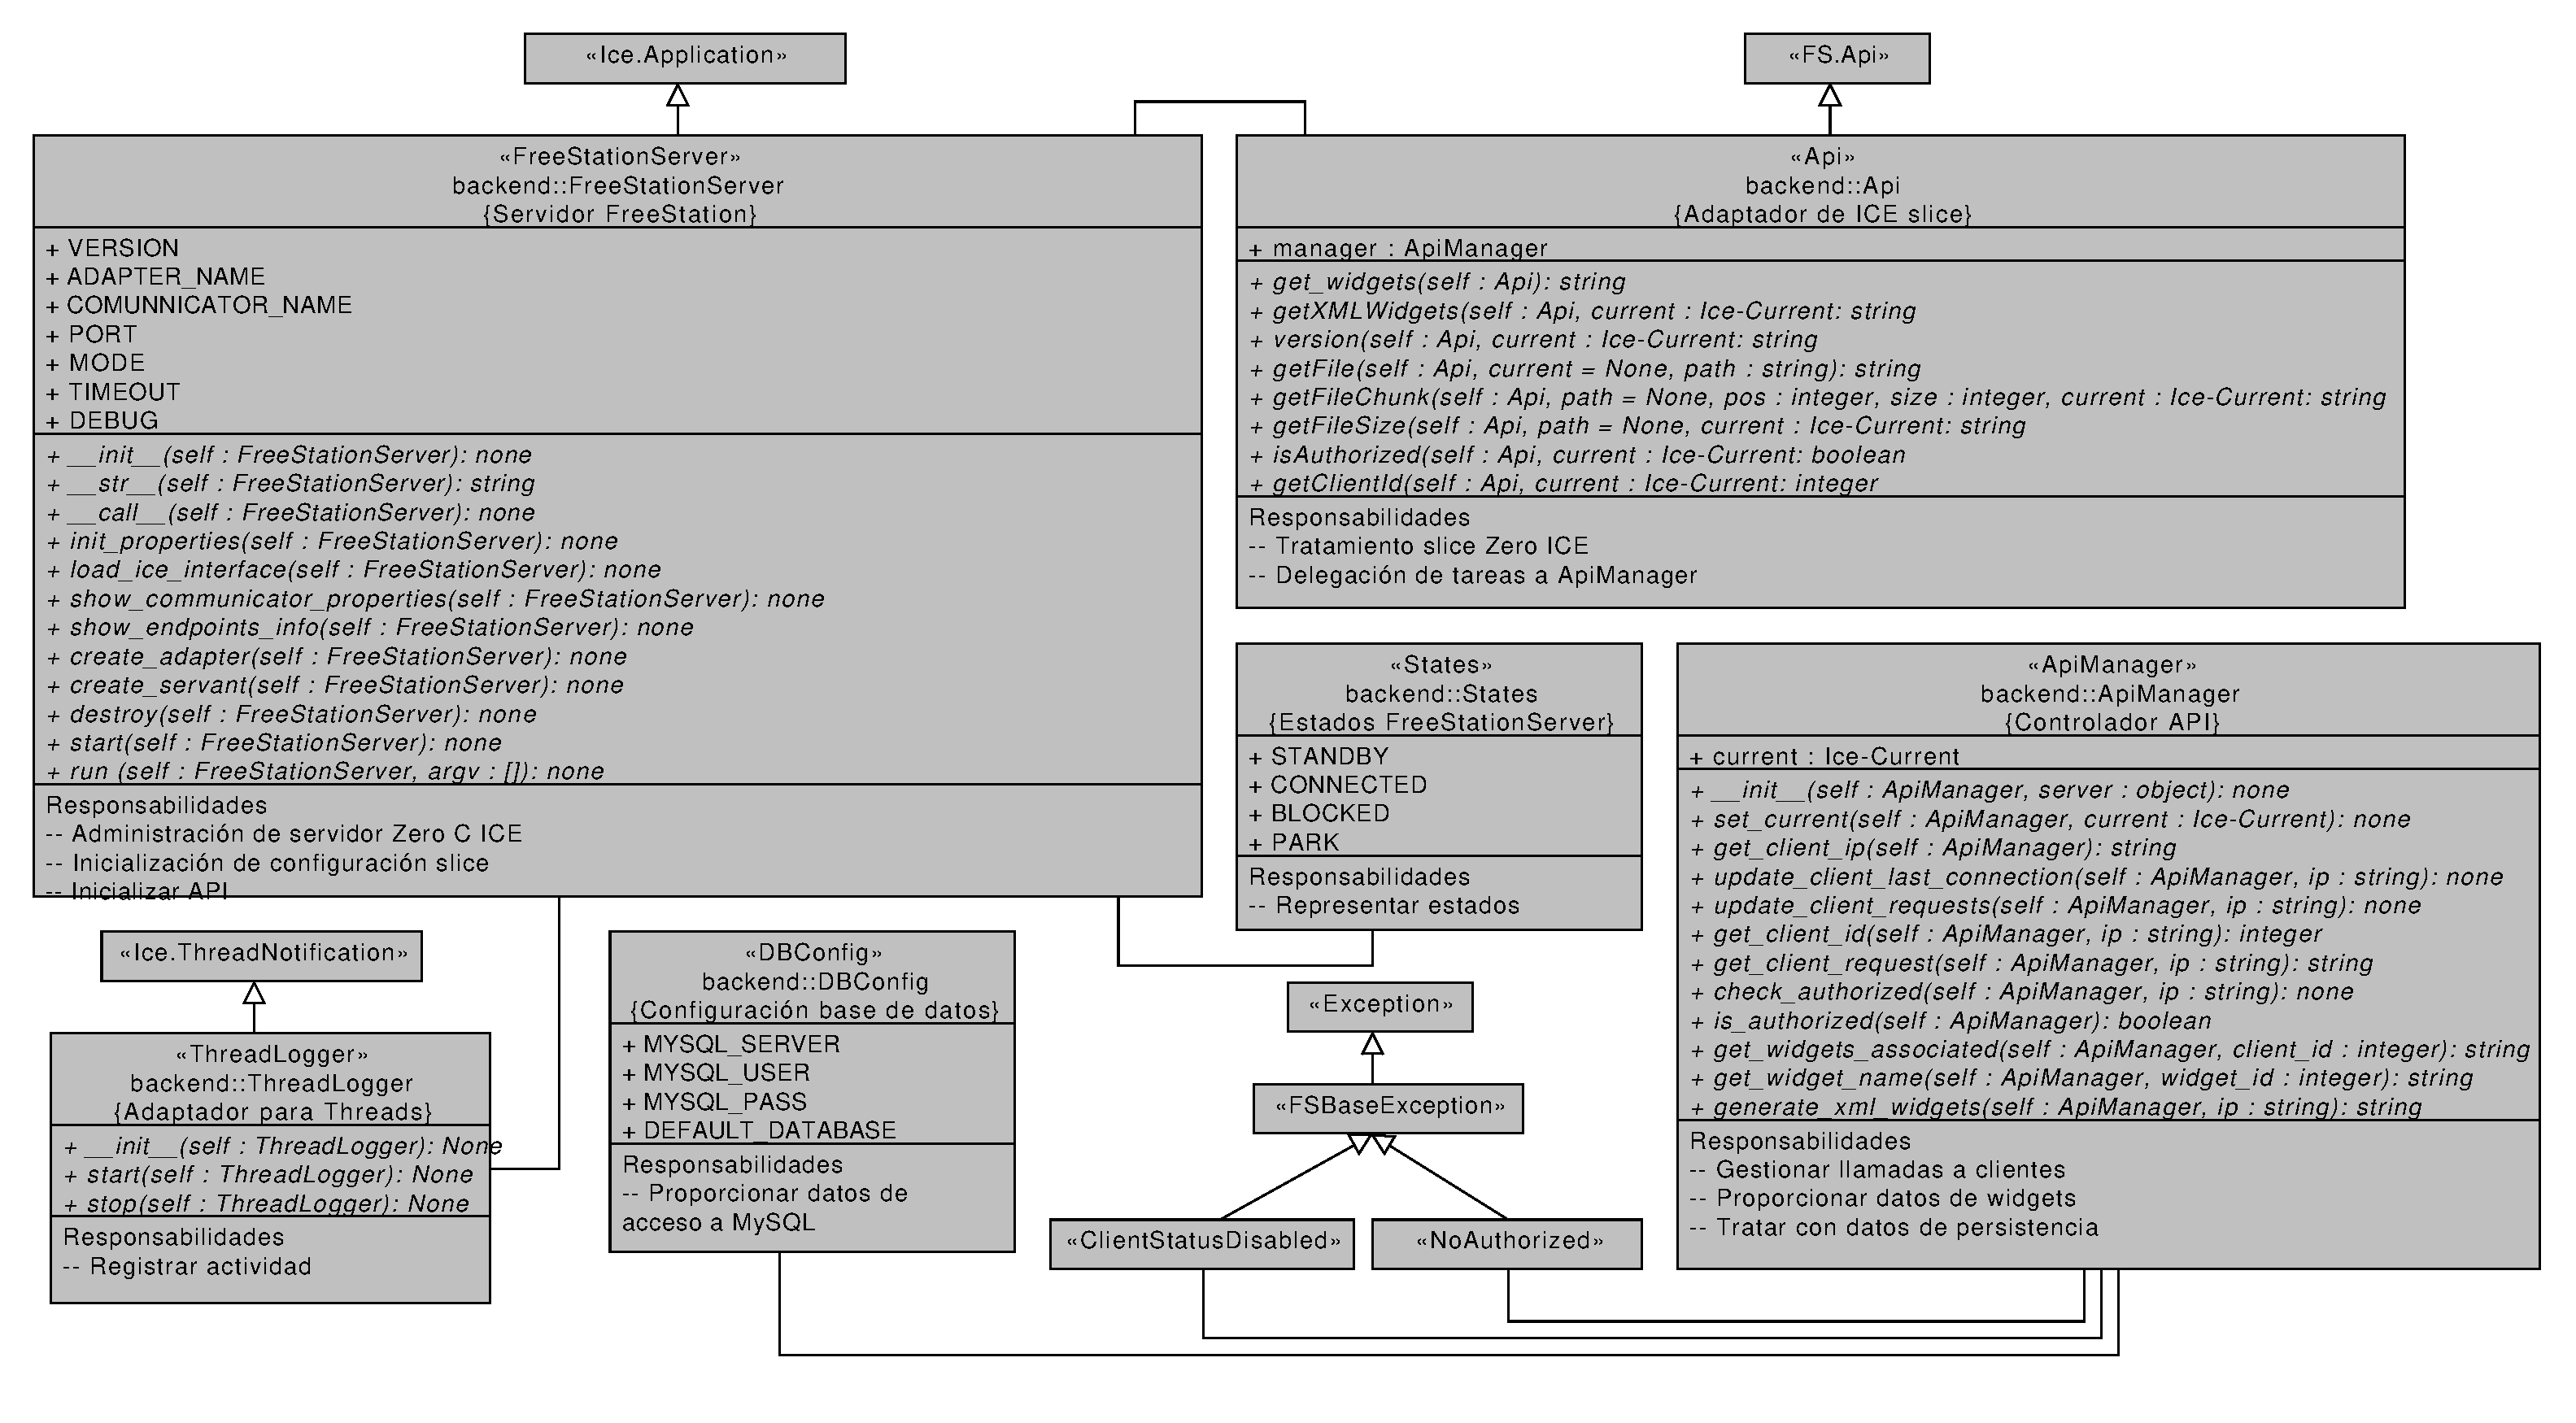
\includegraphics[width=680px,
 height=425px]{src/img/diagrams/freestation-zero-ice-backend.pdf}
 \label{fig:classzeroicebackend}
 }%
{Diagrama de clases para Backend Zero C ICE}{fig:classzeroicebackend}

\newpage

La figura ~\ref{fig:classzeroicebackend} muestra en conjunto el diagrama de
clases implicado en este sistema backend servidor de la aplicación que ha sido
explicado en anteriores secciones.

\subsubsection{Frontend}

El \emph{Frontend} esta basado en PHP y maquetado con HTML\cite{W3C99}, CSS\cite{W3C06}
y Javascript. Es completamente modular y los subsistemas que intervienen están
desacoplados. La forma en la que interactúan los subsistemas es sencilla y
transparente al programador o usuario.

La aplicación web esta orientada a la administración del servidor y
configuración de widgets y clientes. Es una capa de software que facilita la
edición y configuración sencilla. Estas tareas puedan realizarse
generando los datos manualmente, pero conllevan mayor tiempo y complejidad.

Los ejemplos de uso del \emph{Frontend} son detallados en el anexo de Apéndice
B: Manual de usuario. En esta sección se detallará su arquitectura y
funcionamiento para la generación dinámica de interfaces a través de widgets y su comunicación con
backend servidor.

El frontend esta diseñado como una arquitectura con tres
subsistemas o módulos. Estos son: ClientCore, ServerCore y WidgetCore.
Posteriormente un módulo de CMS los conecta y accede a la persistencia de datos
utilizando el patrón \acs{MVC}\label{acro:MVC} como se explico en la sección
~\ref{sec:interfazderivada}. A continuación se detallan los subsistemas.

\textbf{Subsistema de widgets}

Los widgets tienen un peso importante dentro del \emph{Frontend}. Este
subsistema es el encargado de la gestión de operaciones con widgets.

La clase \emph{WidgetCore} escrita en PHP construye las bases para manejar las
operaciones básicas de gestión de widgets. Permite obtener todos los widgets
disponibles en el servidor con el método $getList()$. También puede obtenerse la
configuración de un widget conociendo el identificador numérico y único del
mismo. Para ello se usa la función $get()$. Sin embargo, puede ser necesario
obtener los datos del widget a través del nombre y para ello es necesario la
función $getFromName()$. La comprobación previa de la existencia de un widget
puede realizarse mediante su identificador con la función $exists()$.

Una vez se disponen de los datos necesarios del widget, la clase
\emph{WidgetCore} puede renderizar la información del mismo con el método
$render()$. Para creación de widgets personalizados el programador
sólo debe limitarse a implementar las interfaces de los objetos que desee crear 
y estos serán cargados según su funcionalidad.

\textbf{Subsistema de clientes}

El subsistema de clientes está organizado por la clase \emph{ClientCore}. Esta
clase encapsula el tratamiento y gestión de clientes proporcionando un acceso
sencillo a sus estructuras y datos.

Los métodos de la clase \emph{ClientCore} permiten obtener los datos de un
cliente dado su identificador numérico único con el método $get()$. Comprobar la
existencia de un cliente a través de un identificador con el método $exist()$.
Por otro lado, para obtener la lista de widgets asociados a un cliente se
utiliza el método $getWidgetsAssociated()$ y para comprobar si un widget está
asociado a un cliente $isWidgetsAssociated()$ o borrar un determinado widget de
un cliente con $deleteWidgetsAssociated()$.

Asimismo, un cliente puede darse de baja usando el método delete() y el
identificador de cliente. Es importante recalcar que si el cliente no existe 
la excepción \emph{ClientNoExist} será lanzada. Para habilitar o deshabilitar el
estado de un cliente, se puede proceder al cambio con la función
$changeStatus()$.

\textbf{Subsistema de gestión del servidor}

La gestión del \emph{Frontend} para el servidor se realiza mediante la clase
\emph{ServerCore}. Es un clase núcleo (core) que habilita las funciones más
básicas para operar con el \emph{Backend}. Entre sus operaciones están el inicio
del servidor con la función $start()$, que previamente vaciar los registros de
log con la función privada $resetLogs()$ para iniciar unos nuevos en la
ejecución. La parada del servidor con $stop()$. Para conocer el PID de ejecución
del proceso servidor se proporciona la función $getServerPid()$. Esta función devolverá vacío en caso de no
encontrar un proceso en ejecución.

\newpage

Los registros de log que son almacenados corresponden según el nivel de
importancia del mensaje o si proceden de la salida estándar del proceso o error.

Los niveles asociados son:

\begin{itemize}
    \item \textbf{RUNNING\_LOG}: registro para la salida estándar de
    ejecución. Los datos se almacenan en el fichero running.log.
    \item \textbf{STANDARD\_OUTPUT\_LOG}: registro para la salida estándar
    normal del proceso \emph{Backend} de ICE. Los datos se almacenan en el
    fichero ice\_output.log.
    \item \textbf{STANDARD\_ERROR\_LOG}: registro para la salida estándar de
    error del proceso \emph{Backend} de ICE. Los datos se almacenan en el
    fichero ice\_error.log
    \item \textbf{WARNING\_LOG}: registro para mensajes de aviso en la salida
    estándar. Los datos se almacenan en el fichero ice\_error.log
    \item \textbf{TRACE\_LOG}: registro para mensajes de trazas de depuración en
    la salida estándar. Los datos se almacenan en el fichero ice\_error.log
    \item \textbf{OTHER\_LOG}: registro para otros tipos de mensajes sin
    categorizar en la salida estándar. Los datos se almacenan en el fichero
    ice\_error.log
\end{itemize}

Esta clase es la base de operaciones para una clase de más alto nivel como
\emph{WidgetServer}. Es el ``widget" para la gestión del servidor. Esta clase
actúa como vista para la anterior clase controlador \emph{ServerCore} y 
renderiza los datos de registros de logs en cajas animadas y pestañas. Para ello
se basa en la lectura de ficheros indicados en los anteriores niveles de log y 
los analiza según el tipo de mensaje. Por otro lado, obtiene la representación 
del estado del servidor y datos del PID de proceso, ofreciendo botones de
iniciar, parar o reiniciar el servidor.

\textbf{Subsistema de administración de contenidos}

FreeStation se basa en un framework propio y original para la administración de
contenidos o CMS (Content Management System). Se basa ampliamente en el patrón
de diseño MVC reuniendo en una sola biblioteca las utilidades necesarias. La
clase principal permite abrir y cerrar páginas y centrarse sólo en la vista 
del contenido. Para ello utiliza métodos como $openPage()$ y
$closePage()$. Realiza una carga dinámica de clases en ejecución a través de una
clase \emph{Loader} que detecta en tiempo de ejecución la clase a cargar e
importa el código. De esta forma el programador ahorra tiempo en estructurar 
dependencias o fallos por falta de archivos o módulos.

Para esta carga dinámica se basa en la clase \emph{ClassHash} que es un hash de
nombres de clases apuntando a sus rutas. De esta forma el CMS puede cargar
cualquier clase preestablecida en este hash.
Gracias a esta tecnología, los archivos son precargados rápidamente y se evitan
importaciones de código redundantes. En caso de fallo se lanzará una excepción
como \emph{ClassNotExist} que ayudará al programador a conocer fácilmente que
clase no ha sido añadida.

El CMS también incorpora una gestión de errores en tiempo de ejecución para
errores fatales en PHP. PHP por defecto aborta la ejecución del script en caso
de un error fatal, pero la clase \emph{ErrorManager} activa manejadores para
realizar un tratamiento del error, ya sea archivando el error para posterior
análisis o mostrándolo en pantalla de forma agradable para su depuración.

Para el tratamiento de persistencia el CMS incorpora una clase llamada
\emph{MySqlDriver} que trata con consultas a base de datos. Para limpieza y
seguridad de los datos se incorpora una clase \emph{Sanitizer}. De igual modo
para el tratamiento de sesiones de usuario se incorpora la clase \emph{Session}.

Para la creación de un menú vertical con los distintos apartados la
funcionalidad es ofrecida por la clase \emph{WidgetVerticalMenu}. Cabe destacar
que el desarrollo del \emph{Frontend} es mucho más sencillo a partir del CMS 
propio construido.

Estos subsistemas son el núcleo del \emph{Frontend} del servidor web y permiten
realizar todas las operaciones de forma básica e independiente. De este modo, la estructura
de un subsistema permite un uso completamente modular del mismo, pudiéndose
reutilizar en otras partes de la aplicación. Por otro lado, es posible añadir
más funcionalidad sin tener que cambiar ninguna otra parte de la arquitectura.
Como conjunto inicial, estos subsistemas cubren la mayoría de las
necesidades básicas.

El siguiente diagrama de clases muestra las utilidades que brinda el sistema
en conjunto y sus subsistemas para el \emph{Frontend}.

\newpage

\hvFloat[
 floatPos=!htb,
 capWidth=h,
 capPos=r,
 capAngle=90,
 objectAngle=90,
 capVPos=c,
 objectPos=c]{figure}{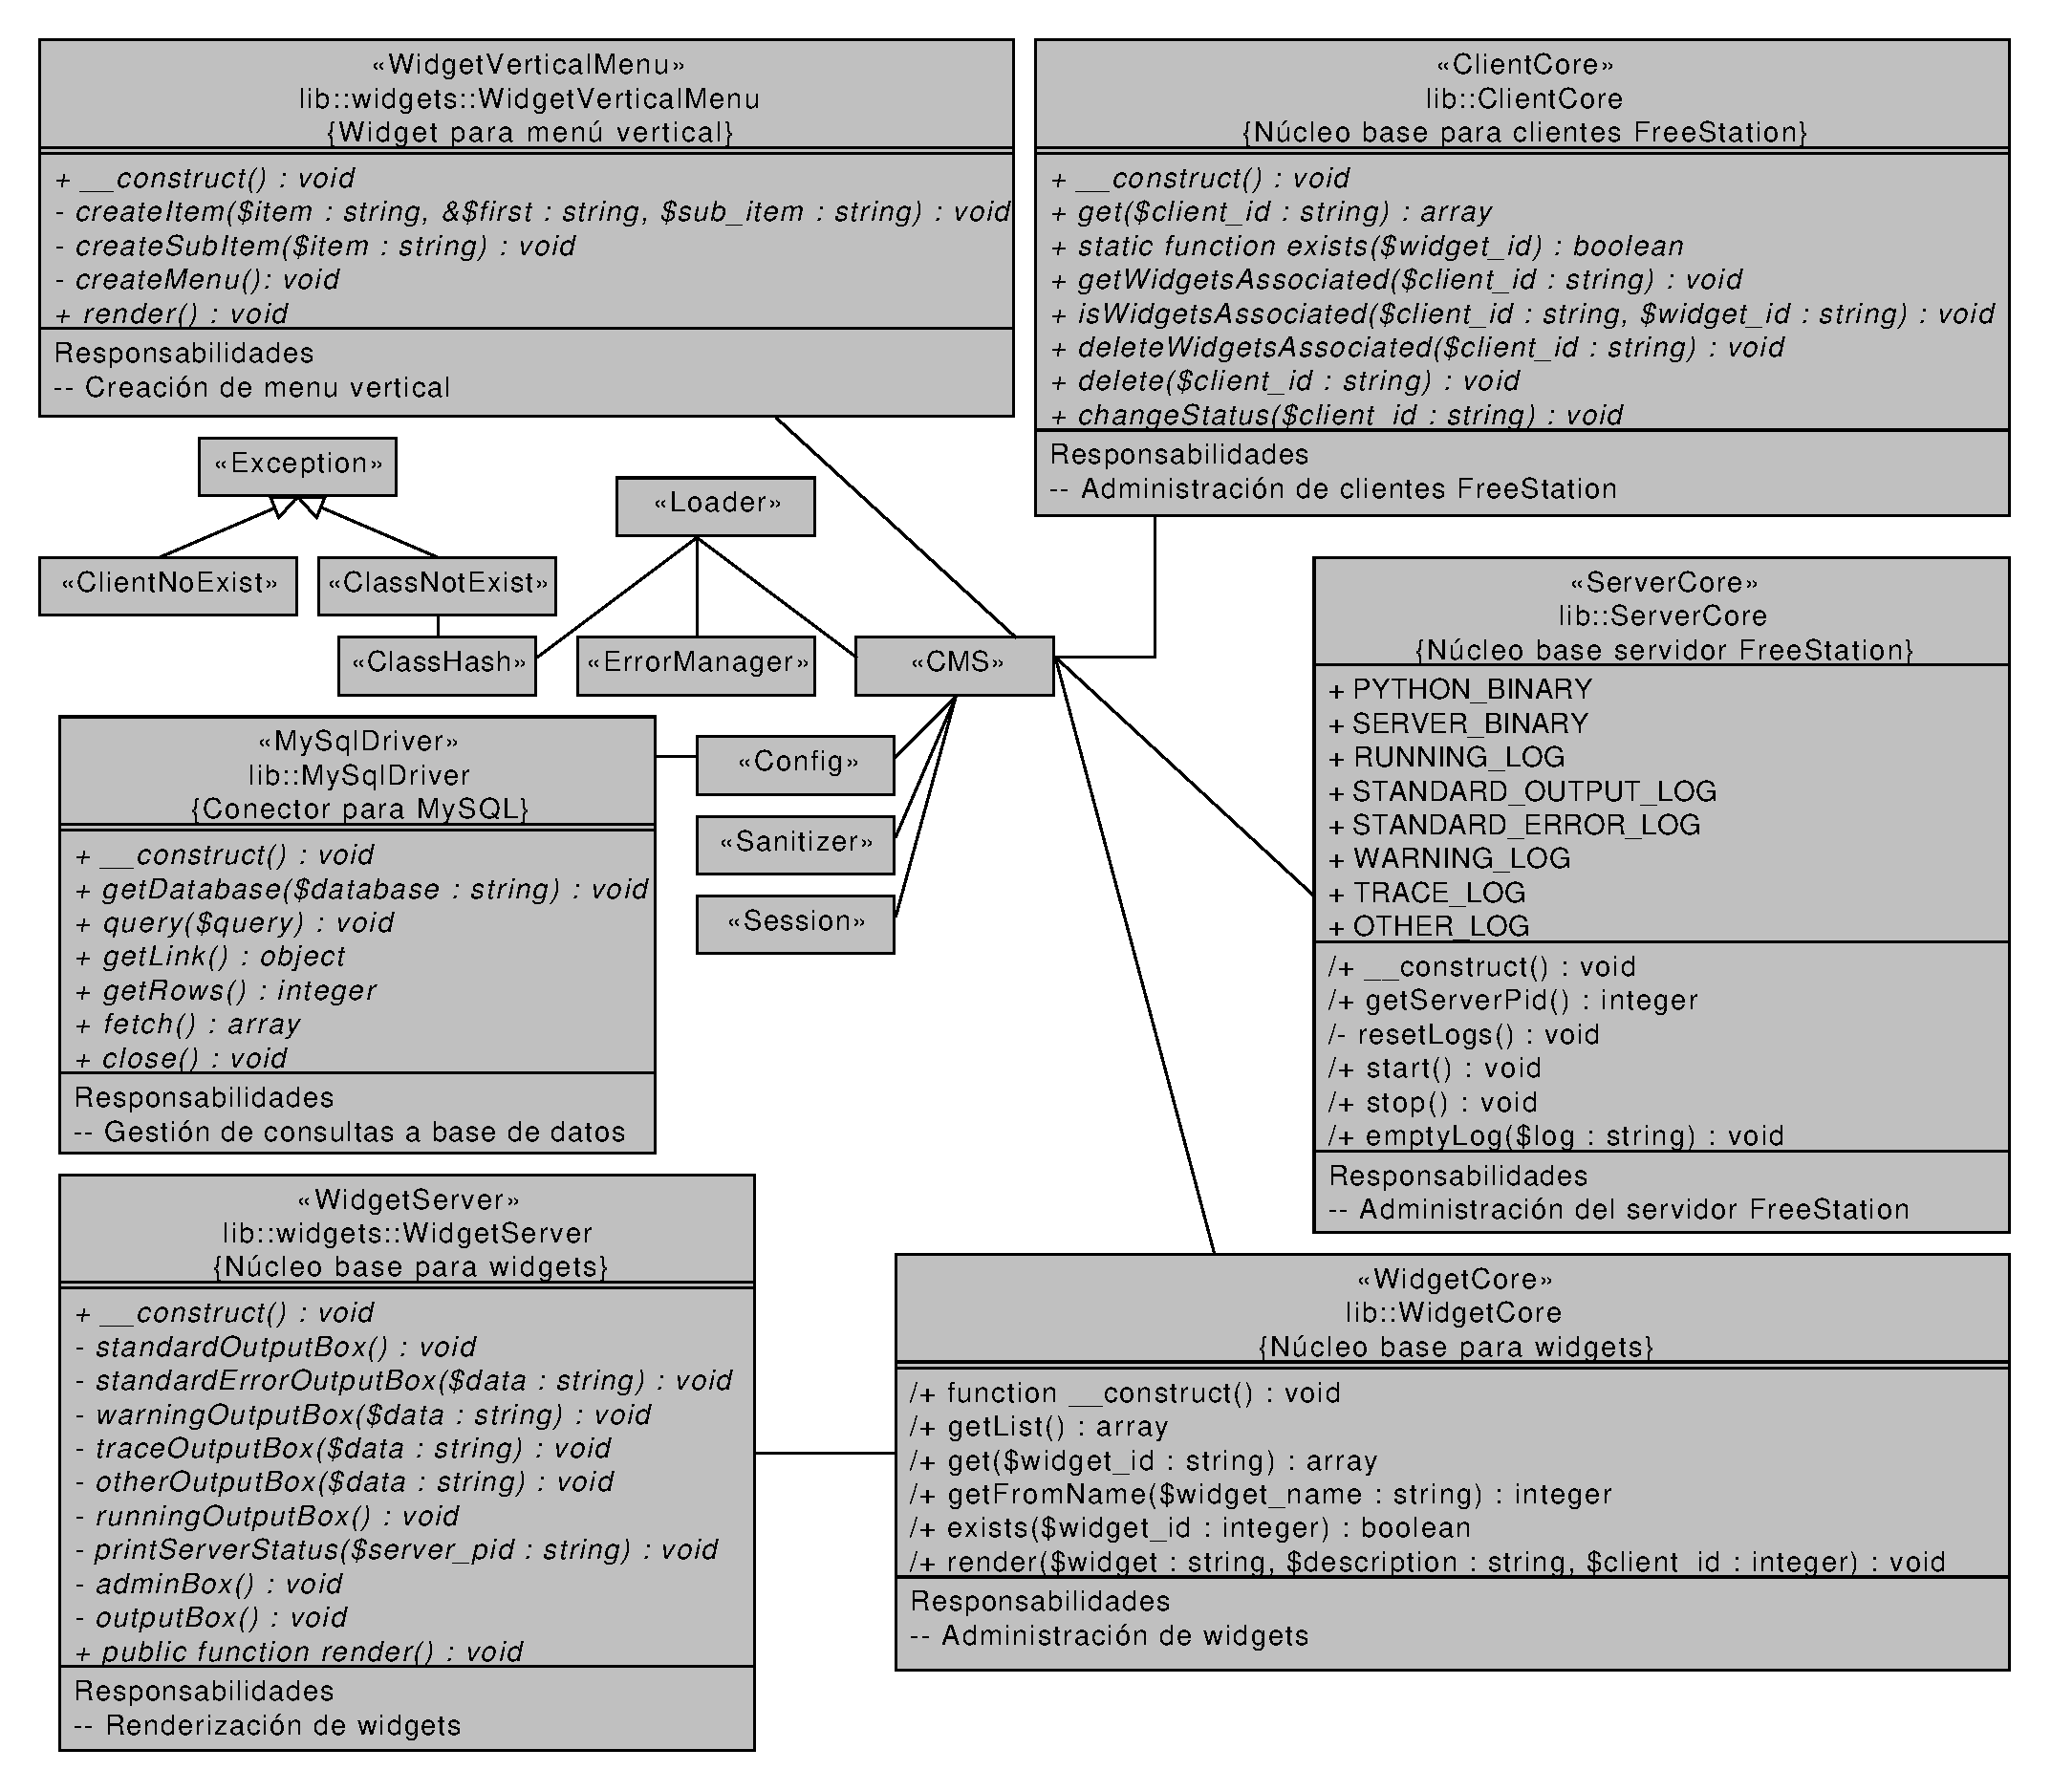
\includegraphics[width=680px,
 height=425px]{src/img/diagrams/freestation-frontend-php-diagram.pdf}}%
{Diagrama de clases para Frontend PHP}{fig:classfrontendphp}

\newpage

\section{\uppercase{Capa de persistencia}}

En la capa de persistencia se usa un servidor de base de datos MySQL 5.1 para
almacenar los resultados no volátiles.

Todos los datos almacenados han utilizado el motor de almacenamiento
InnoDB\footnote{InnoDB:
\url{http://dev.mysql.com/doc/refman/5.1/en/innodb-storage-engine.html}} de
MySQL de manera transaccional.

El diagrama ERR tiene el aspecto siguiente:

\begin{figure}[ht]
    \begin{center}
        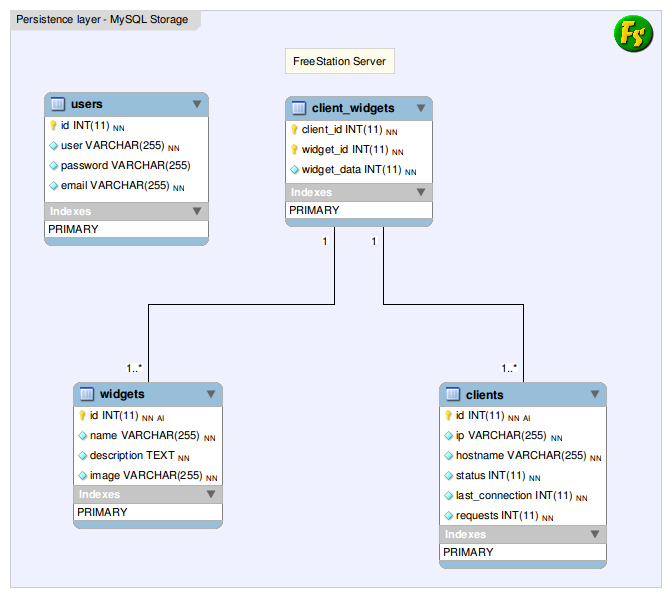
\includegraphics[scale=0.68]{src/img/diagrams/mysql-database.png}
        \caption[Diagrama ERR]
          {Diagrama ERR}
    \end{center}
\end{figure}

\newpage

Se pueden apreciar 4 tablas diferentes.

\begin{itemize}
  \item Tabla usuarios: es la encargada de almacenar los datos de los usuarios
  que acceden a la aplicación frontend mediante sus credenciales.
 
  Se almacenan datos como usuario, contraseña y email. La contraseña es cifrada
  con el algoritmo \acs{SHA}\label{acro:SHA}-1\footnote{SHA-1: Secure Hash
  Algorithm es cifrado por funciones hash seguro \url{http://www.ietf.org/rfc/rfc3174.txt}}

  \item Tabla clientes: se guardan los datos pertenecientes a clientes
  Freestation. Cada cliente posee un identificador único e IP permitida
  para el acceso. Puede asociarse un alias como hostname para fácil
  identificación humana. Se guardan datos como última conexión y número de
  peticiones realizadas en total.

  \item Tabla widgets: almacena los widgets existentes en el servidor con
  un identificador único, nombre, descripción e imagen.
  
  \item Tabla clientes-widgets: utilizada para almacenar las relaciones entre
 widgets asociados a clientes y datos personalizados por cada widget.
\end{itemize}

\section{\uppercase{Arquitectura Apache CouchDB}}
\label{sec:couchdbapache}
CouchDB™ es una base de datos documental basada en JSON, que permite realizar
consultas MapReduce mediante Javascript y dispone de una API REST normalizada
que puede ser gestionada mediante el protocolo HTTP\footnote{Wiki CouchDB:
\url{http://wiki.apache.org/couchdb/}} (veáse la sección ~\ref{sec:apirest}).

Su desarrollo está orientado totalmente a recursos web\cite{AnJ10}. Funciona
incluso en aplicaciones móviles. El acceso a documentos se realiza generalmente mediante un
navegador web vía HTTP. Las consultas combinadas transforman los documentos con
Javascript.

La sincronización y replicación están integradas
por defecto. Para ello, utiliza una replicación incremental para distribuir los
datos eficientemente, soportando incluso configuraciones de maestro-maestro 
con detección automática de conflictos. 

La configuración maestro-maestro permite que dos instancias CouchDB repliquen
los mismos datos de forma sincronizada para obtener una alta disponibilidad y
como solución ante fallos de caídas por un único nodo. De esta forma, si un nodo
couchDB se pierde, siempre existe una copia exacta y original en otro nodo.

Por otro lado, permite un alto número de particiones para
datos siendo consistente en todo momento con los datos proporcionados. La
tolerancia de fallos está asegurada anteponiendo los datos como objetivos de
mayor prioridad dentro del flujo de la aplicación.
Por otro lado, habilita una consola web a modo de interfaz llamada Futon que 
permite una cómoda depuración\footnote{Proyecto CouchDB:
\url{http://couchdb.apache.org}}. 

Su principal objetivo es operar en entornos distribuidos de datos orientados a
aplicaciones web. Los cambios, al ser replicados constantemente, permiten un
alto grado de fiabilidad. Para ello dispone de la habilidad realizar cambios offline.
La ventaja de operar de esta forma, es ser más tolerante a fallos y permitir
cambios offline que sean sincronizados en el momento que sea posible.

Por este motivo, la adopción de CouchDB se ha hecho muy popular en aplicaciones
web basadas en HTML 5.

\subsection{Propagación de señales en CouchDB}
\label{sec:signalscouch}

La interfaz (GUI) y el cliente FreeStation no se comunican directamente entre
sí. Aunque es posible realizar una codificación directa, la configuración de
Webkit para la interfaz HTML no puede enviar señales de forma cómoda al 
cliente FreeStation basado en GTK. El mecanismo base, es la ejecución y 
evaluación por retrollamadas de Webkit basadas en javascript. Para su 
recepción, el código javascript debe ser evaluado en el
cliente FreeStation y analizado detallamente. Este enfoque hace complicado el
mantenimiento y añadir nuevo código siendo poco escalable en el tiempo.

Por ello se adapta un enfoque de una aplicación intermediaria. En este enfoque
se utilizan la emisión de señales a través de CouchDB.
CouchDB escucha estas señales y las propaga como eventos en ambas 
direcciones\footnote{Couchbase Client Library Python 1.0:\\
\url{http://www.couchbase.com/docs/couchbase-sdk-python-1.0/index.html}}.

\newpage

\begin{figure}[ht]
    \begin{center}
        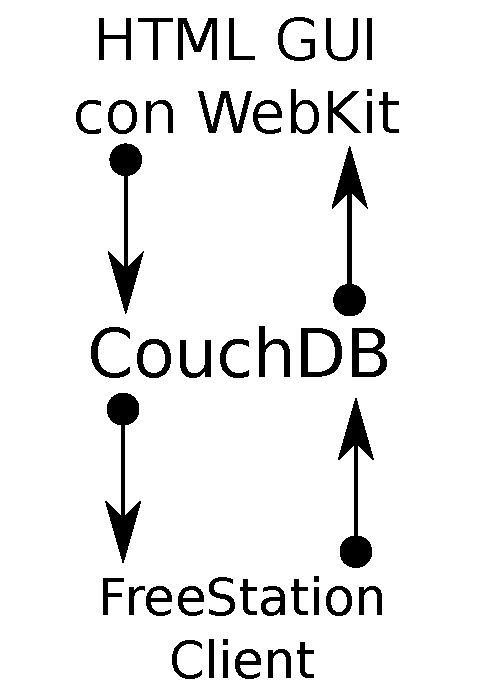
\includegraphics[scale=0.5]{src/img/diagrams/event-propagation.pdf}
        \caption[Propagación de eventos y señales en CouchDB]
          {Propagación de eventos y señales en CouchDB}
          \label{fig:couchdbevent}
    \end{center}
\end{figure}

La figura ~\ref{fig:couchdbevent} muestra el flujo de propagación de señales
explicado anteriormente. 

\begin{figure}[hb]
    \begin{center}
        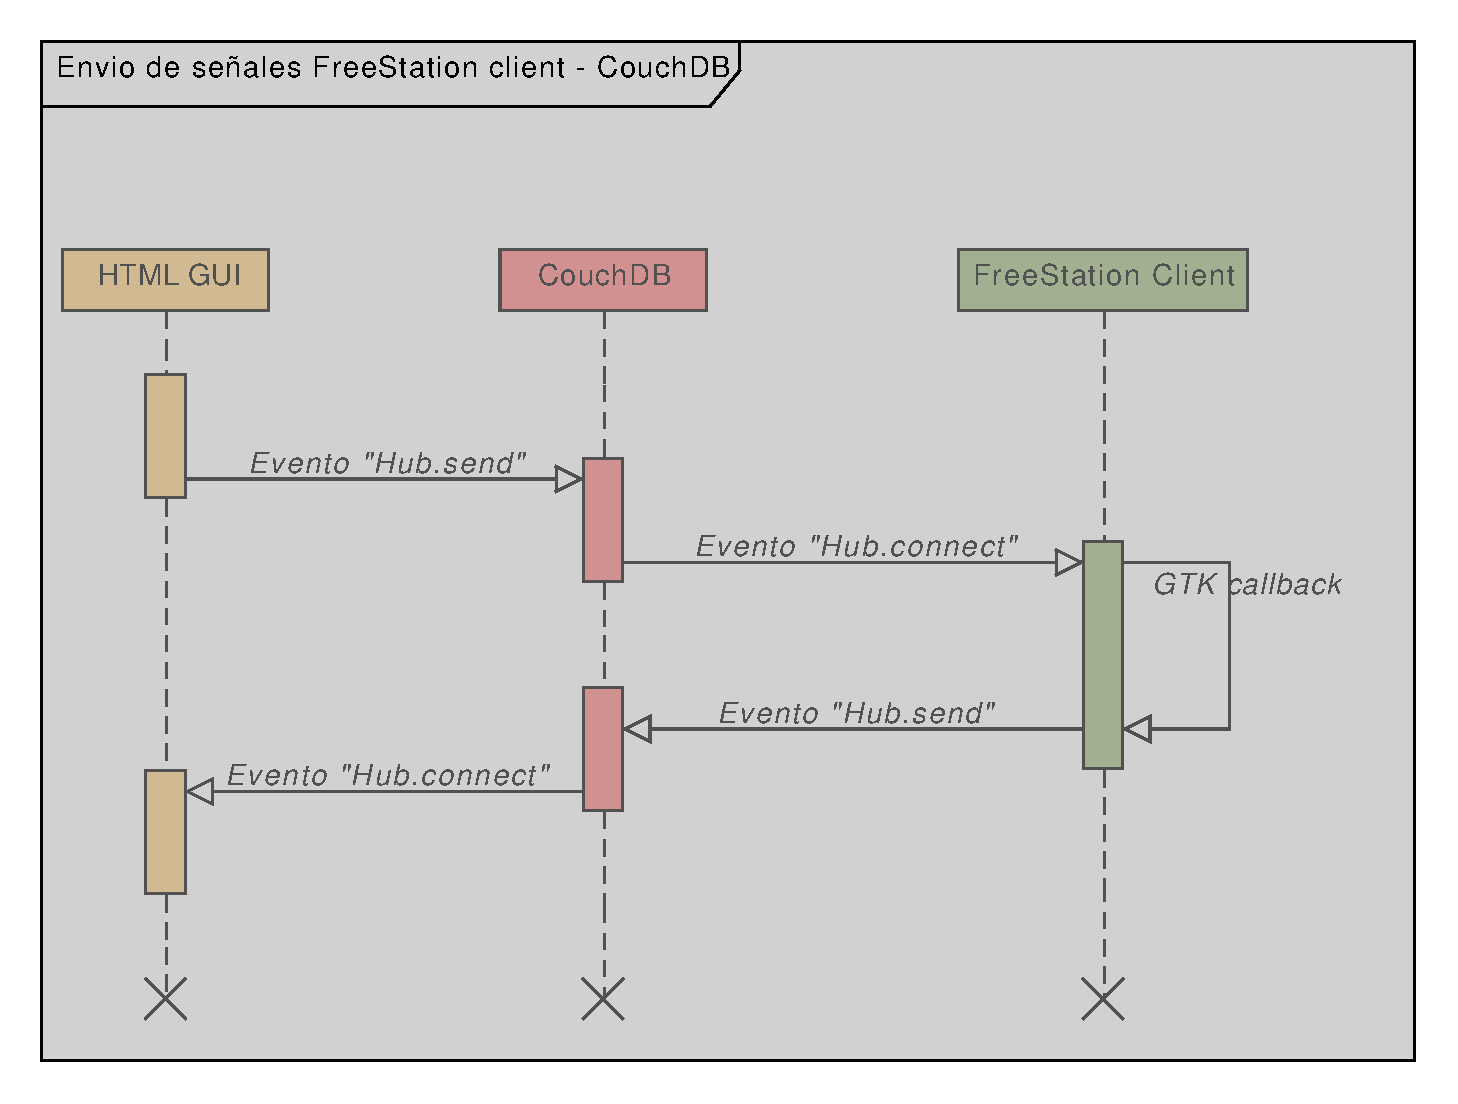
\includegraphics[width=325px]{src/img/diagrams/freestation-seq-diagram-couchdb.pdf}
        \caption[Diagrama secuencia entre componentes] {Diagrama secuencia entre componentes}
          \label{fig:secuenciacouch}
    \end{center}
\end{figure}

\newpage
El diagrama de secuencia explicado por la figura ~\ref{fig:relationscouch}
muestra la especificación de llamadas entre componentes y las señales emitidas y
recibidas. El componente Hub o concentrador sirve de mediador entre componentes.
Las señales del hub como send() permiten enviar los datos y el tipo de señal.
Estas a su vez son conectadas en el componente (ya sea en javascript para html,
python en couchdb o python en GTK).

\subsection{Diagrama de clases para CouchDB}
\label{sec:classforcouchdb}
Las clases de código que intervienen en el proceso son principalmente la
interfaz GTK del cliente FreeStation que iniciara la incorporación e importación de un
widget basado en CouchDB. Dicho widget conectara sus señales GTK para 
mantenerse a la espera de nuevos eventos. Posteriomente inicializará un
wigdet browser que permite carga la composición de arranque de una interfaz
HTML5 basada en elementos web.

En ese momento una instancia de CouchDB con un usuario único se creará de forma
transparente en la aplicación y adoptará las señales que fueron conectadas
anteriormente. Con propósitos de depuración, se iniciara un analizador 
(inspector) a modo consola web.

Paralelamente se pondrá a la escucha un widget DBus para otros widgets como
MountDetector, para detectar cambios de hardware como dispositivos USB.

Una vez están preparados estos componentes, la interacción en la interfaz basada
en HTML5 estará a la espera de eventos de usuario.

Una vez se produzcan como se ha comentado en el apartado ~\ref{sec:signalscouch}
la clase Hub iniciará una factoría de señales en HubFactory y los datos podrán
ser recibidos mediante la clase DataProvider. La interacción encapsulada de la
clase Hub, permitirá conectar con la biblioteca Microfiber y la biblioteca
javascript main.js de la interfaz HTML5.

\newpage

\hvFloat[
 floatPos=!htb,
 capWidth=h,
 capPos=r,
 capAngle=90,
 objectAngle=90,
 capVPos=c,
 objectPos=c]{figure}{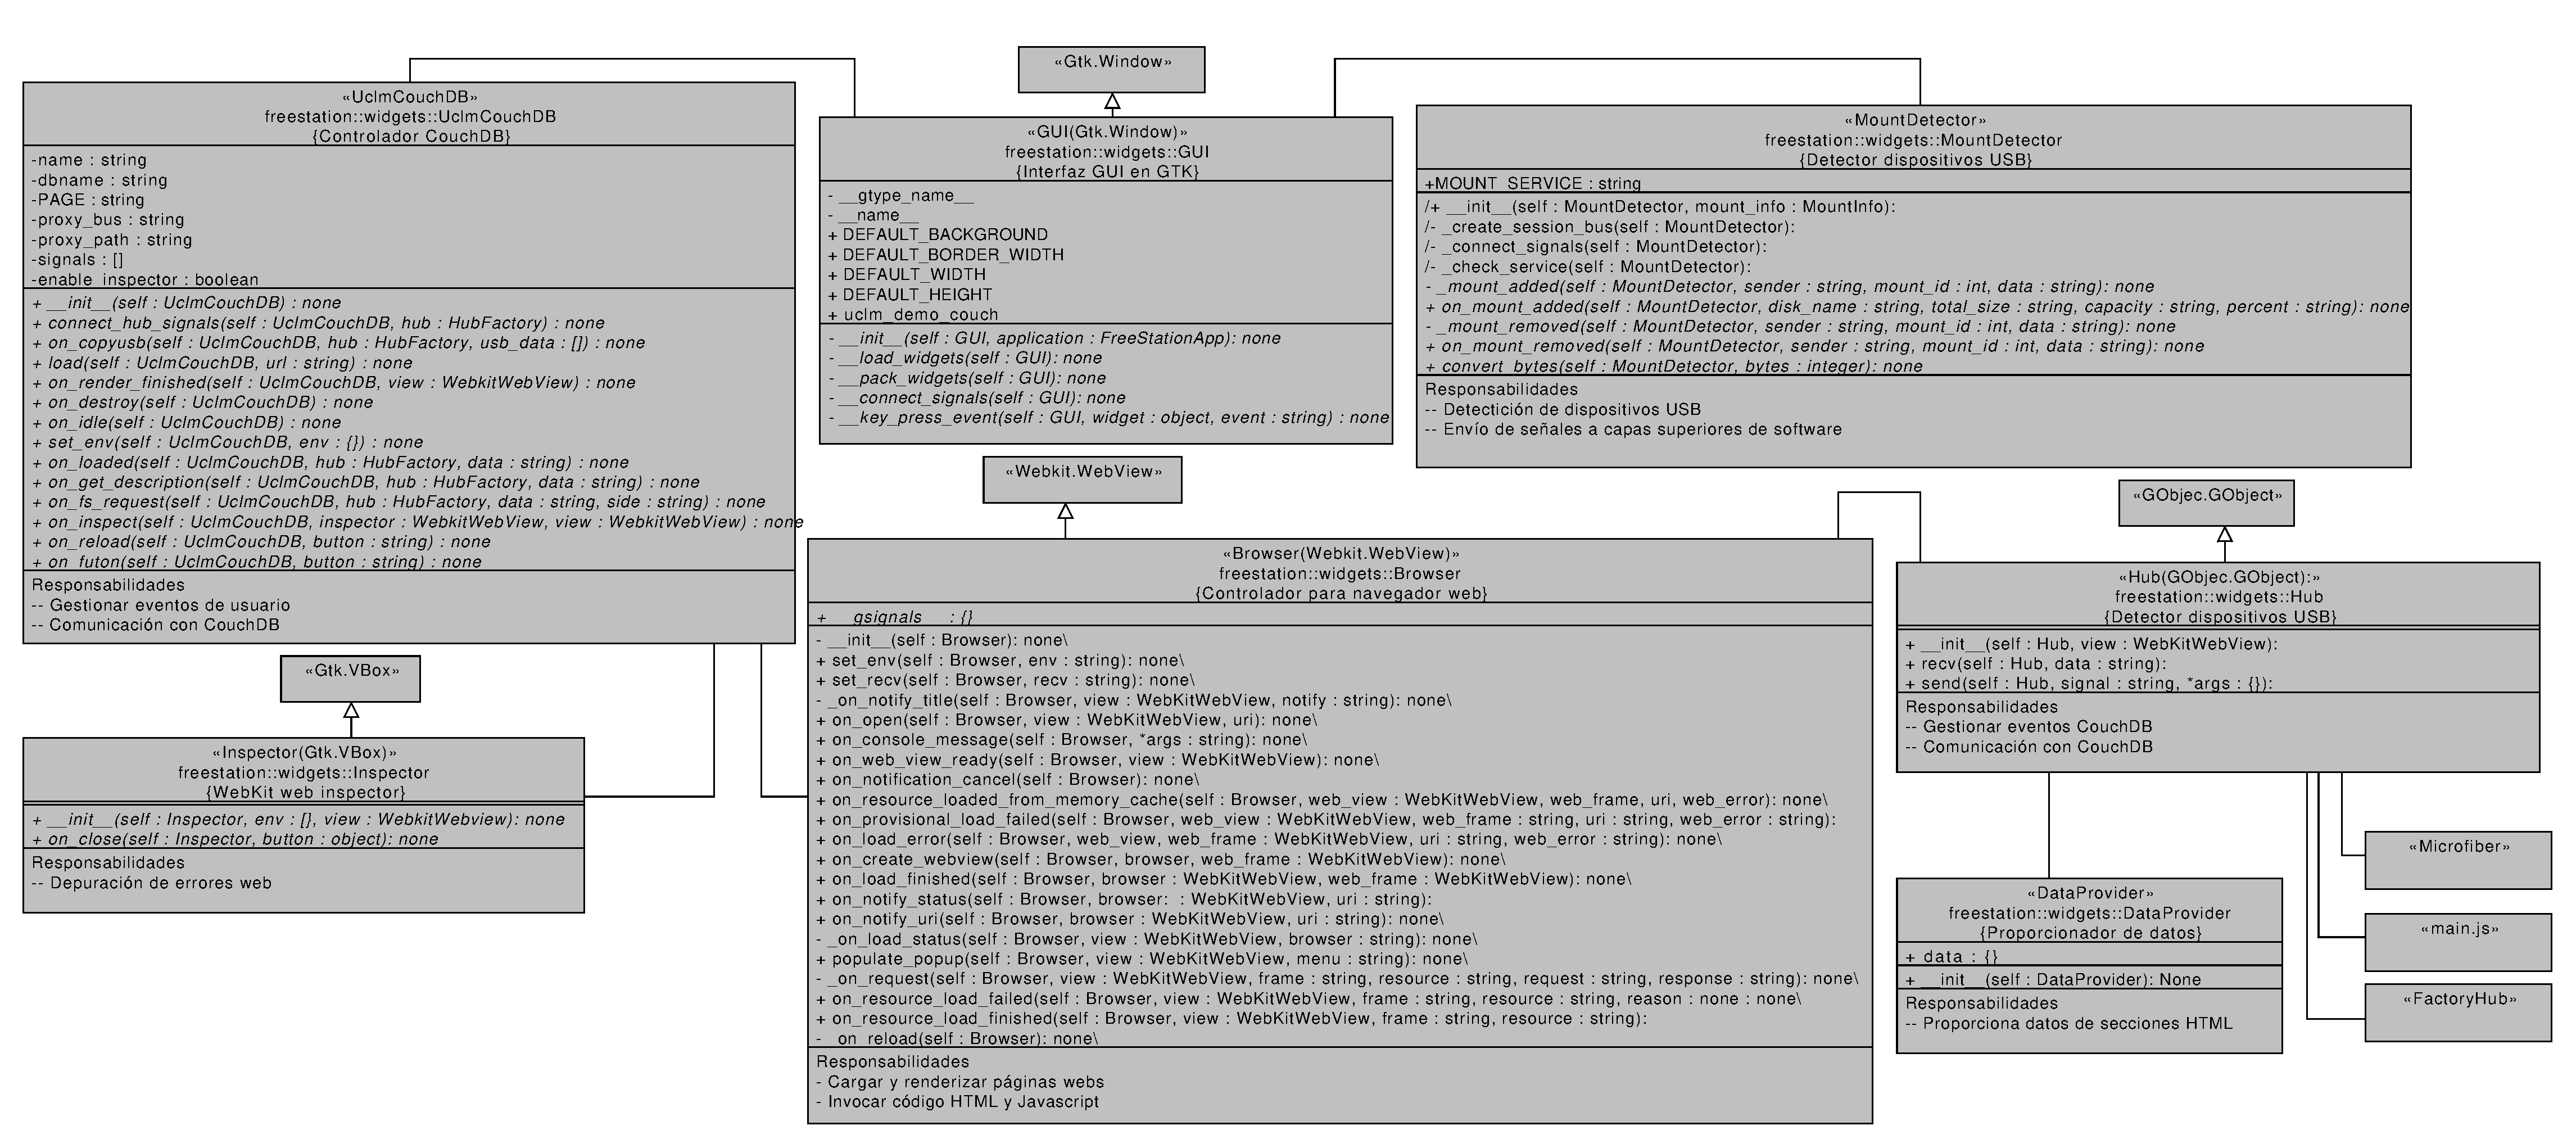
\includegraphics[width=680px,
 height=425px]{src/img/diagrams/freestation-class-diagram-couch.pdf}}%
{Diagrama de clases para CouchDB}{fig:classcouch}

\newpage

Las ventajas de la utilización de CouchDB es la realización y maquetación de
aplicaciones basadas en HTML5. El enriquecimiento de la interfaz abre más
posibilidades de interacción con el usuario y el acercamiento a interfaces
más naturales (NUI) (véase sección ~\ref{sec:interfazNUI}). Al contrario que
los elementos GTK, permite una mayor personalización en la apariencia de la
aplicación. El prototipado por tanto es mucho más rápido y permite esbozar la
aplicación con poco esfuerzo para el desarrollador.

El enfoque orientado a eventos y señales permite abstraer por capas la aplicación
y reutilizar código entre diferentes módulos o widgets.

El problema de este enfoque es conocer la latencia
entre un cambio realizado por la interfaz, el procesado de CouchDB y su 
recepción por parte del cliente. En el peor escenario, el cliente también 
podría emitir una señal de vuelta a la interfaz a través de CouchDB, lo que
completaría el ciclo de interacción.

Según se comentó en las sección ~\ref{sec:generacionint} era
crítico que la respuesta ante la interacción del usuario esté totalmente 
acotada, y en un tiempo mínimo para que la percepción del usuario fuera óptima.

Según la ejecución del fichero benchmark.py basado en el módulo cProfile de
Python, el arranque en frío de aplicación conlleva 57106 llamadas de
funcione primitivas. Estas son en su mayoría importaciones del módulo gnome
instrospection de bindings. Esta ejecución toma un tiempo total de 1,267 segundos.
Las funciones primitivas implicadas en freestation son 1756, tomando únicamente
un tiempo de 0,145 segundos.

Cada evento y señal procesado de CouchDB conlleva un tiempo de procesado de
0,019 segundos. 

Por tanto, para reducir la latencia del sistema, CouchDB se focaliza en la 
concurrencia. Para que el sistema sea lo suficientemente escalable, se
deben tratar con tres principales tipos de problemas:

\begin{itemize}
    \item Peticiones de lectura
    \item Peticiones de escritura
    \item Volumen de datos
\end{itemize}

\begin{figure}[ht!]
   \centering
   %%----primera subfigura----
   \subfloat[]{
        \label{fig:latency:a}         %% Etiqueta para la primera subfigura
        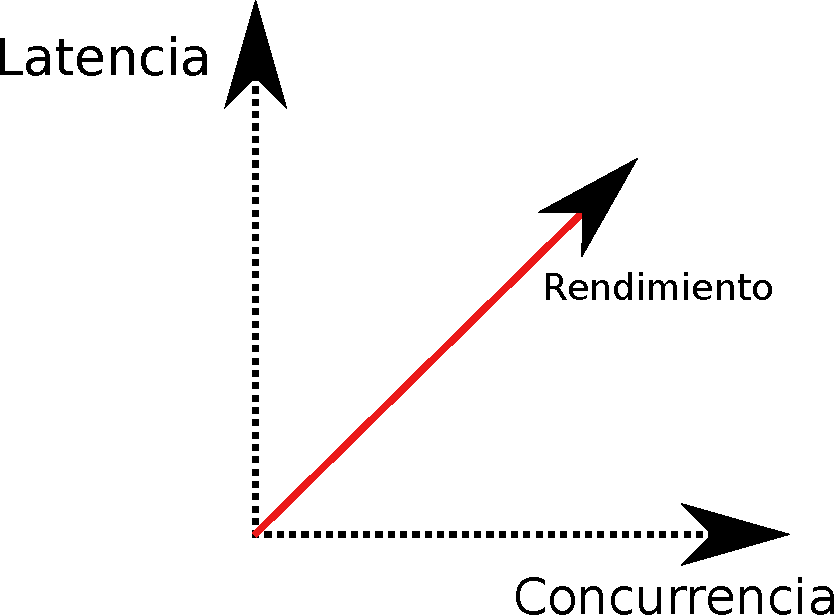
\includegraphics[width=0.38\textwidth]{src/img/diagrams/latency-concurrency.pdf}}
   \hspace{0.1\linewidth}
   %%----segunda subfigura----
   \subfloat[]{
        \label{fig:reads:b}         %% Etiqueta para la segunda subfigura
        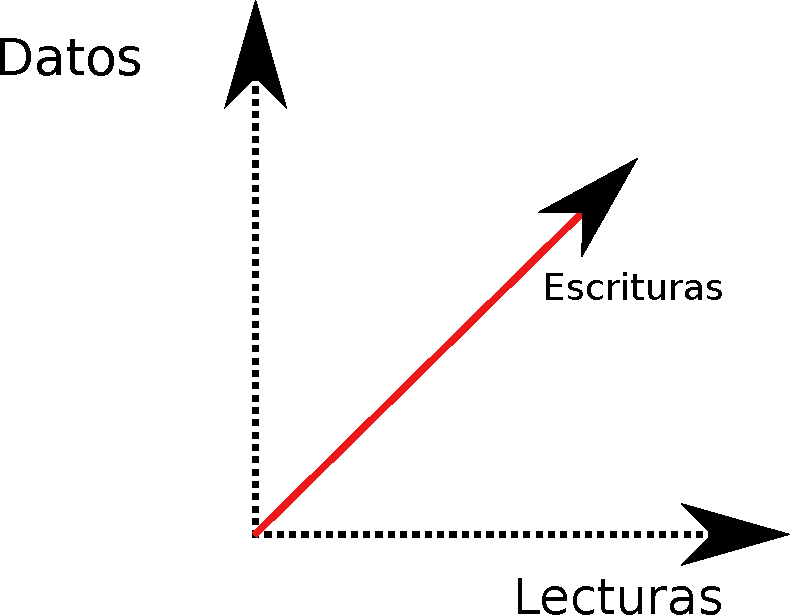
\includegraphics[width=0.38\textwidth]{src/img/diagrams/read-writes.pdf}}\\[20pt]
        \caption{a) Relación entre latencia y concurrencia b) Relación entre datos y
    lecturas}
   \label{fig:relationscouch}    
\end{figure}

\newpage

La figura ~\ref{fig:relationscouch} muestra la relación explicada en CouchDB. En
general el sistema será más fiable con un menor número de atributos entre las
señales y cuando estas puedan paralerizarse. CouchDB es flexible en 
ese aspecto y permite construir bloques de datos para resolver un problema
exacto.

De esta forma, las señales permiten acciones que interactuaran en flujo HTML
emitido desde Javascript al motor de WebKit. El bucle de ejecución sera
procesado con CouchDB y será recibido en una aplicación cliente basada en
GTK como FreeStation.

Así, gracias a esta solución, se obtienen las siguientes ventajas frente a un 
desarrollo basado en aplicaciones de escritorio puras:

\begin{itemize}
  \item Mayor facilidad en el diseño del interfaz.
  \item Total flexibilidad a la hora de modificar el interfaz ``al vuelo en
tiempo de ejecución''
  \item Posibilidad de reutilizar la amplia gama de componentes diseñados en
HTML.
  \item La información es fácilmente organizable estructurando contenidos en
 JSON como formato estándar.
  \item Desarrollo totalmente multiplataforma, sin necesidad de desarrollar
  bindings propios
 \item Combinación de presentación y navegación de la aplicación en un mismo
estándar basado en HTML 5.
 \item Simplicidad y coherencia con principios fundamentales para el desarrollo
de una interfaz efectiva (véase sección ~\ref{sec:guiadesignpoi}).
\end{itemize}

\subsubsection{API REST en CouchDB}
\label{sec:apirest}

La API REST de CouchDB es gestionada mediante el protocolo HTTP. Para ello
utiliza un método de almacenamiento de información basado en documentos, es
decir, una gestión documental. El atributo DocID identifica de forma única un
documento.

Algunos ejemplos de acceso a documentos únicos:

\begin{lstlisting}[language={bash}, texcl=false, caption={Ejemplo 1 CouchDB}]
http://localhost:5984/prueba/algun_id
\end{lstlisting}

\begin{lstlisting}[language={bash}, texcl=false, caption={Ejemplo 2 CouchDB}]
http://localhost:5984/prueba/otro_id
\end{lstlisting}

\begin{lstlisting}[language={bash}, texcl=false, caption={Ejemplo 3 CouchDB}]
http://localhost:5984/prueba/BA1F48C5418E4E68E5183D5BD1F06476
\end{lstlisting}  

Las anteriores url mostradas apuntan al identificador del documento. De esta
forma pueden accederse a documentos con una simple URL y mediante HTTP\footnote{CouchDB HTTP document API:\\
\url{http://wiki.apache.org/couchdb/HTTP_Document_API}}..

\begin{lstlisting}[language={bash}, texcl=false, caption={Petición HTTP}]
curl -X GET 'http://localhost:5984/prueba/algun_id?rev=3243'
\end{lstlisting}

Un documento CouchDB es simplemente un objeto JSON, con cualquier estructura o
anidamiento posible. Algunos atributos como el número de revisión se guardan de
forma adicional.

\begin{lstlisting}[language={bash}, texcl=false, caption={Ejemplo Documento
CouchDB}]
{
 "_id":"freestation_widgets",
 "_rev":"D1C946B7",
 "load":true,
 "maximize":false,
 "allocation":[0, 0, 800, 600],
 "wigets": [
   {"Name":"MountInfo", "Enabled":True, "Depends":"MountUSBStorage"},
   {"Name":"VideoArea", "Disabled":True} ]
}
\end{lstlisting}

Los atributos que preceden por ``'\_' son reservados para uso de CouchDB.

\subsection{Cliente ligero microfiber}

Microfiber\footnote{Proyecto Microfiber:
\url{https://launchpad.net/microfiber}} es una biblioteca con el propósito de adaptador genérico para hacer
peticiones HTTP con datos JSON en la API REST de CouchDB\footnote{Documentación de Microfiber:
\url{http://docs.novacut.com/microfiber/index.html}}.

Es una API orientada a una gran cantidad de métodos excepcionales que permite
realizar llamadas de forma sencilla, abstrayendo la complejidad de CouchDB.

Según la ejecución del fichero benchmark\_microfiber.py la cantidad de
lecturas/escrituras/borrados/guardados es aproximadamente de 140 por segundo, lo
que garantiza una gestión eficiente de los recursos:

\begin{lstlisting}[language={bash}, texcl=false, caption={Benchmark Microfiber}]
Benchmarking microfiber *** Python: 3.2.3, i686, Linux
  Saving 2000 documents in db 'test_benchmark_microfiber'...
    Seconds: 16.21
    Saves per second: 123.4
  Getting 2000 documents from db 'test_benchmark_microfiber'...
    Seconds: 7.91
    Gets per second: 253.0
  Deleting 2000 documents from db 'test_benchmark_microfiber'...
    Seconds: 17.73
    Deletes per second: 112.8
Total seconds: 41.84
Total ops per second: 143.4
\end{lstlisting}

Su principal ventaja y motivo de uso es la abstracción del capturar el entorno
(enviroment) de CouchDB. El entorno se compone de la url de acceso, con
los credenciales en base64 para autenticación básica en OAuth de HTTP.
Por tanto microfiber lidia con los pequeños detalles de la conexión con CouchDB.

Otro punto a favor es que permite instancias por usuario (\emph{per user single
based}) o como sistema completo (\emph{per system based}).

Por otro lado, Microfiber también permite llevar a cabo acciones a nivel de base
de datos para CouchDB usando la instancia del servidor CouchDB.

\section{\uppercase{Caso de explotación POI UCLM}}

Con el fin de ilustrar un ejemplo funcional, se desarrolló un caso de
explotación basado en un POI para la UCLM siguiendo las guías de diseño de
interfaces según la sección ~\ref{sec:guiadesignpoi}.
En este caso de explotación personalizado, se pretende que los alumnos 
dispongan de un POI con  fácil acceso para descargas de software libre,
distribuciones de sistemas operativos, apuntes, transparencias 
u otros programas de utilidad según el proceso de distribución de POIs de la
sección ~\ref{sec:distributionaccesspoi}.

A través de un Widget llamado UclmDemoCouch se implementa una interfaz
completamente basada en HTML5, CSS 3 y javascript que es renderizada por el
motor web WebKit\footnote{Biblioteca UserWebkit:
\url{https://launchpad.net/userwebkit}}.

A diferencia de los widgets basados en GTK permite utilizar degradados css en
la interfaz, border redondeados en elementos y potenciar un diseño líquido para
distintas resoluciones. Todos los recursos utilizados pueden ser cargados
localmente a través de CouchDB y mediante Microfiber comunicar la interfaz 
con CouchDB para obtener y recibir señales y datos en el cliente FreeStation,
de esta forma se cumple con un patrón MVC como fue explicado en la sección
~\ref{sec:generacionint}.

En el caso de explotación, se permite la copia de software seleccionado a una
unidad USB. Para su detección la interfaz se comunica con CouchDB para que el
cliente FreeStation se ponga a la escucha y monitorice eventos de hardware
mediante DBus.
 
\newpage Todo el desarrollo se ejecuta en Python 3 mediante
bindings a cada biblioteca necesitada.

\begin{figure}[ht]
    \begin{center}
        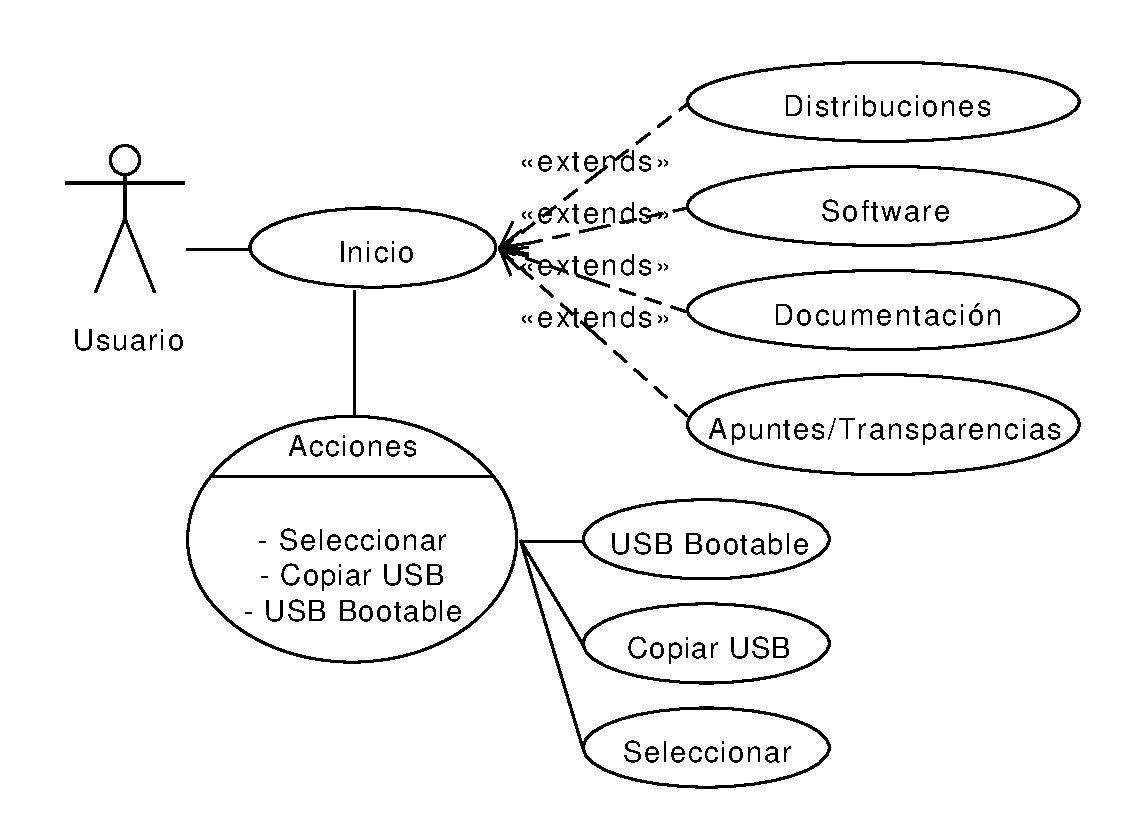
\includegraphics[scale=0.6]{src/img/diagrams/study-case-diagram.pdf}
        \caption[Diagrama de 
        casos de uso para caso de explotación]
          {Diagrama de 
        casos de uso para caso de explotación}
        \label{fig:caseusediagram}
    \end{center}
\end{figure}

En la figura ~\ref{fig:caseusediagram} se detalla el diagrama de casos de usos
para el caso de explotación con sus diferentes acciones implicadas.

\newpage

\subsection{Caso de explotación basado en GTK}
\label{sec:casestudygtk}

El caso de explotación basado en GTK fue desarrollado inicialmente como un
prototipo funcional de aplicación. Este era completo y ofrecía buen rendimiento
y desempeño, pero la apariencia no resultaba demasiado óptima.

\begin{figure}[ht]
    \begin{center}
        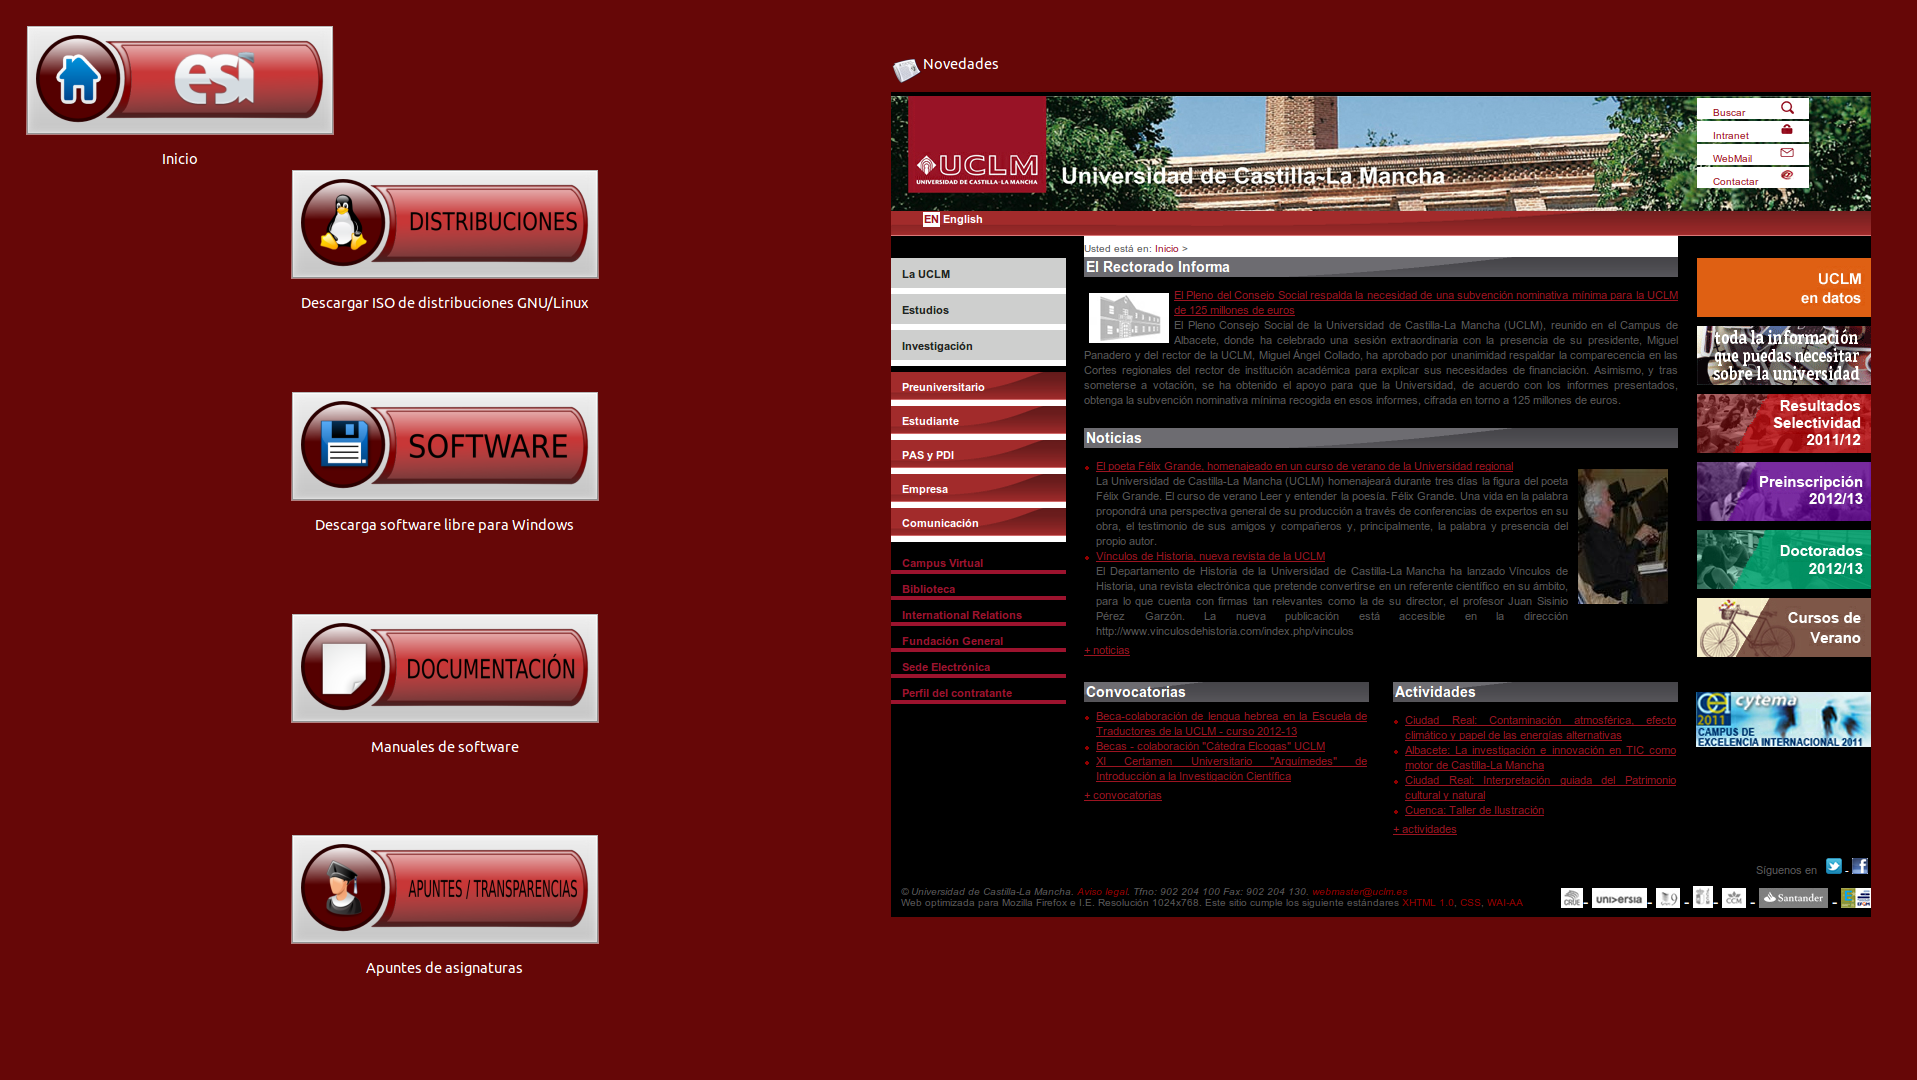
\includegraphics[width=425px]{src/img/freestation-demo1.png}
        \caption[Caso de explotación basado en GTK - Vista inicial]
          {Caso de explotación basado en GTK - Vista inicial}
          \label{fig:explotationgtkinit}
    \end{center}
\end{figure}

La figura ~\ref{fig:explotationgtkinit} muestra la interfaz de bienvenida del
POI desarrollado como ejemplo para la UCLM. La interfaz no seguía algunos de los
patrones NUI definidos en la sección ~\ref{sec:generacionint}. El theming en GTK
era complicado y no permitía características avanzadas como bordes redondeados 
de cajas, degradados lineares en fondos o animaciones de interacción.

El fondo de los botones no admitía efectos de hover con opacidad y no podía
establecerse como transparente. Si podía optarse por establecer el mismo color
del fondo de la aplicación, pero el efecto botón seguía vigente. El diseño por
su parte aunque utilizaba el sistema de cajas de GTK verticales y horizontales
sin posicionamientos absolutos, no era muy adaptable a resoluciones diferentes,
por lo que no disponía de un diseño líquido teniendo el programador la 
responsabilidad de adaptar los widgets a la resolución presente.

La documentación de GTK es bastante completa pero sufre un vacío en el theming
siendo bastante complicado su desarrollo sin ejemplos avanzados. Por otro lado
los bindings a python estan poco probados en dicha competencia y a menudo tienen
errores de programación que no permiten realizar los cambios o no funcionan
correctamente.

\newpage

\begin{figure}[ht]
    \begin{center}
        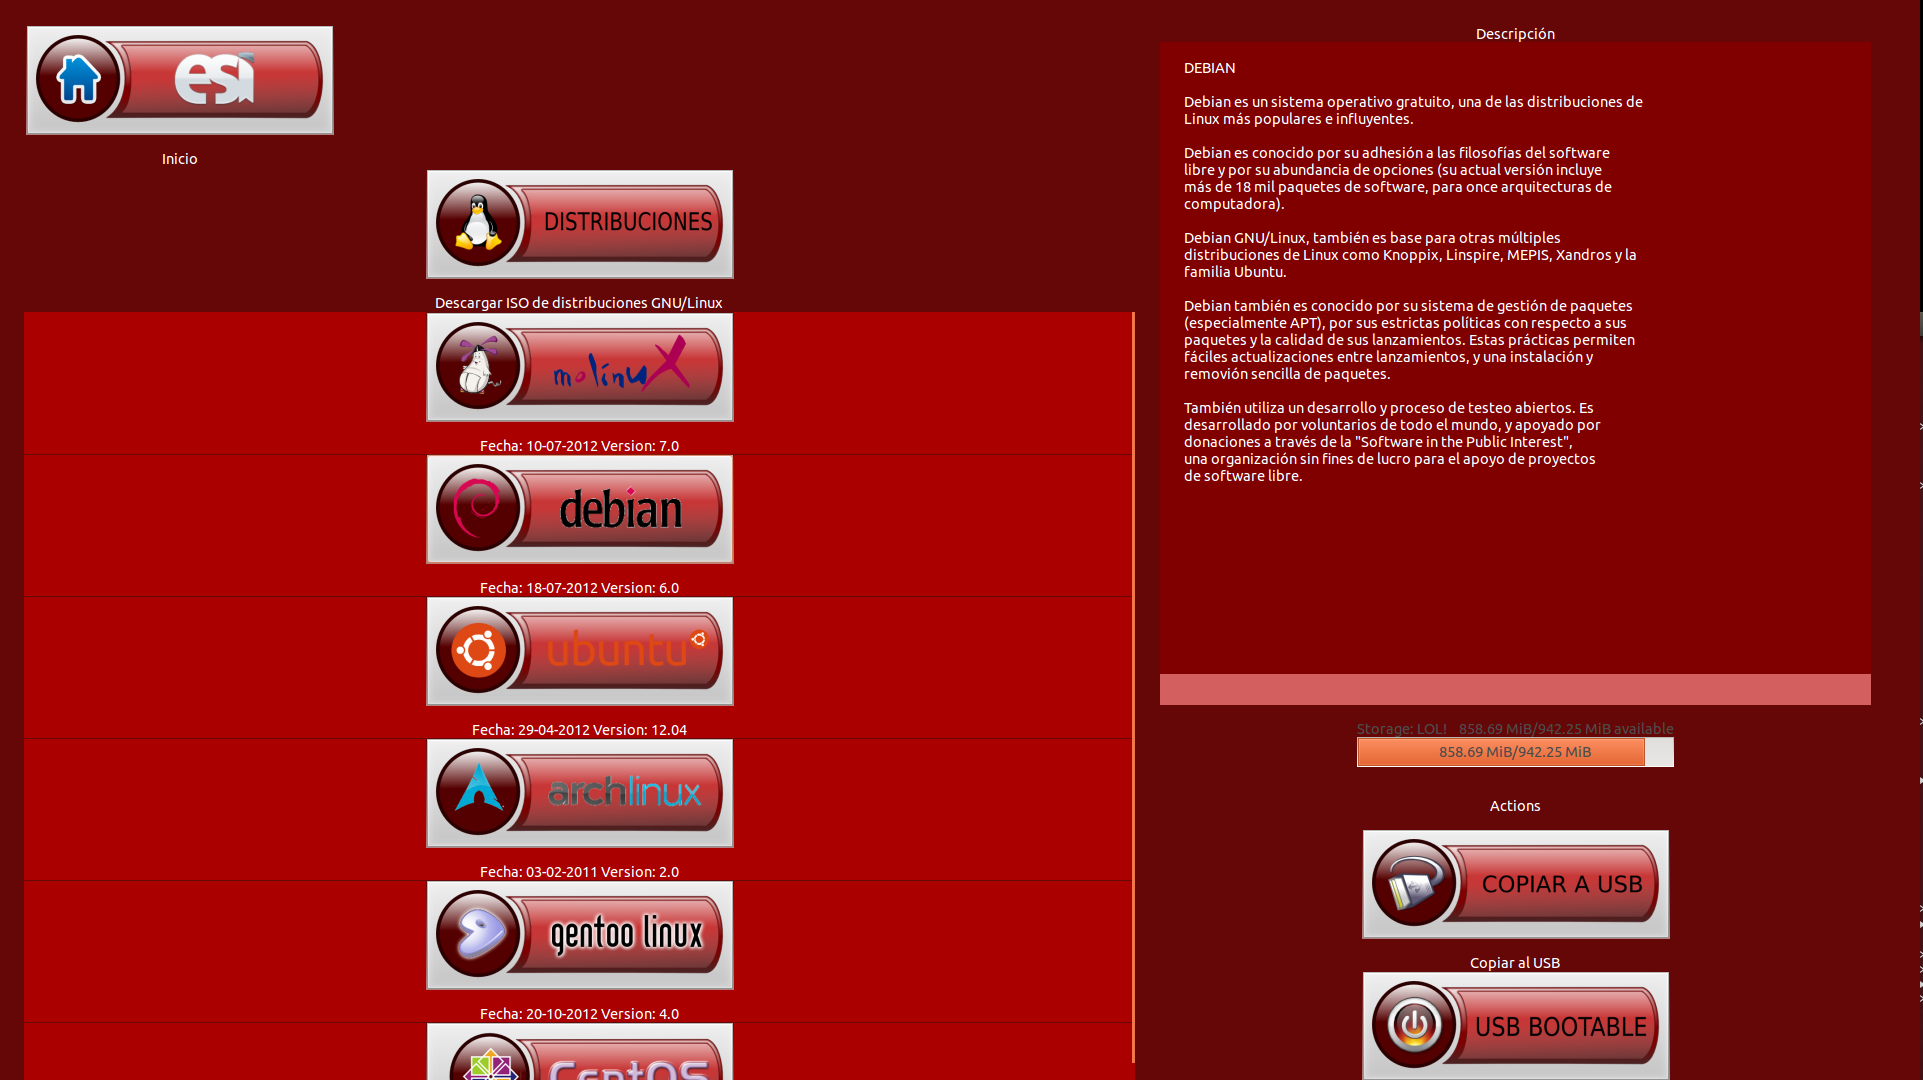
\includegraphics[width=425px]{src/img/freestation-distro-buttons.png}
        \caption[Caso de explotación basado en GTK - Vista de distribuciones]
          {Caso de explotación basado en GTK - Vista de distribuciones}
          \label{fig:distroviewgtk}
    \end{center}
\end{figure}

La vista de distribuciones de la figura ~\ref{fig:distroviewgtk} tenía
problemas similares con las vistas de despegables en scroll y los botones no 
eran adaptables en el contenido. La posibilidad de incorporar estados a botones
seleccionados era complicada y requería la inserción dinámica de widgets, 
destruyendo anteriores. La programación de la interfaz era complicada ya que el
programador debe estar pendiente del modelo de widgets a mostrar y ocultar en
cada interacción de la aplicación.

Por estas razones, se investigaron nuevas tecnologías para la generación
dinámica de interfaces como fue explicado en la sección de antecedentes
~\ref{sec:generacionint} y se intento aplicar un enfoque basado en CouchDB en
combinación de WebKit. Este enfoque requería más investigación y esfuerzo que
GTK pero prometía un gran cambio de resultados en la apariencia y mayor
versatilidad en programación del mismo.

Los anteriores widgets basados en GTK se mantuvieron como presentación del
esfuerzo realizado y como futuro aprovechamiento para otras implementaciones de
widgets que todavía basaran su diseño en GTK.

\newpage

\subsection{Caso de explotación basado en CouchDB}

El caso de explotación basado en CouchDB tuvo inicialmente una curva de
aprendizaje bastante elevada. Se basaba en una tecnología reciente y poco usada
por empresas o programadores independientes.

Gracias al contacto de varios desarrolladores, conversaciones en IRC y
consultas directas al código fuente, la comprensión de la tecnología fue más
rápida adquiriendo un mayor nivel de la misma.

El resultado, fue la realización de una aplicación notablemente diseñada con
mejor apariencia y más adaptada a las reglas NUI. 

\begin{figure}[ht]
    \begin{center}
        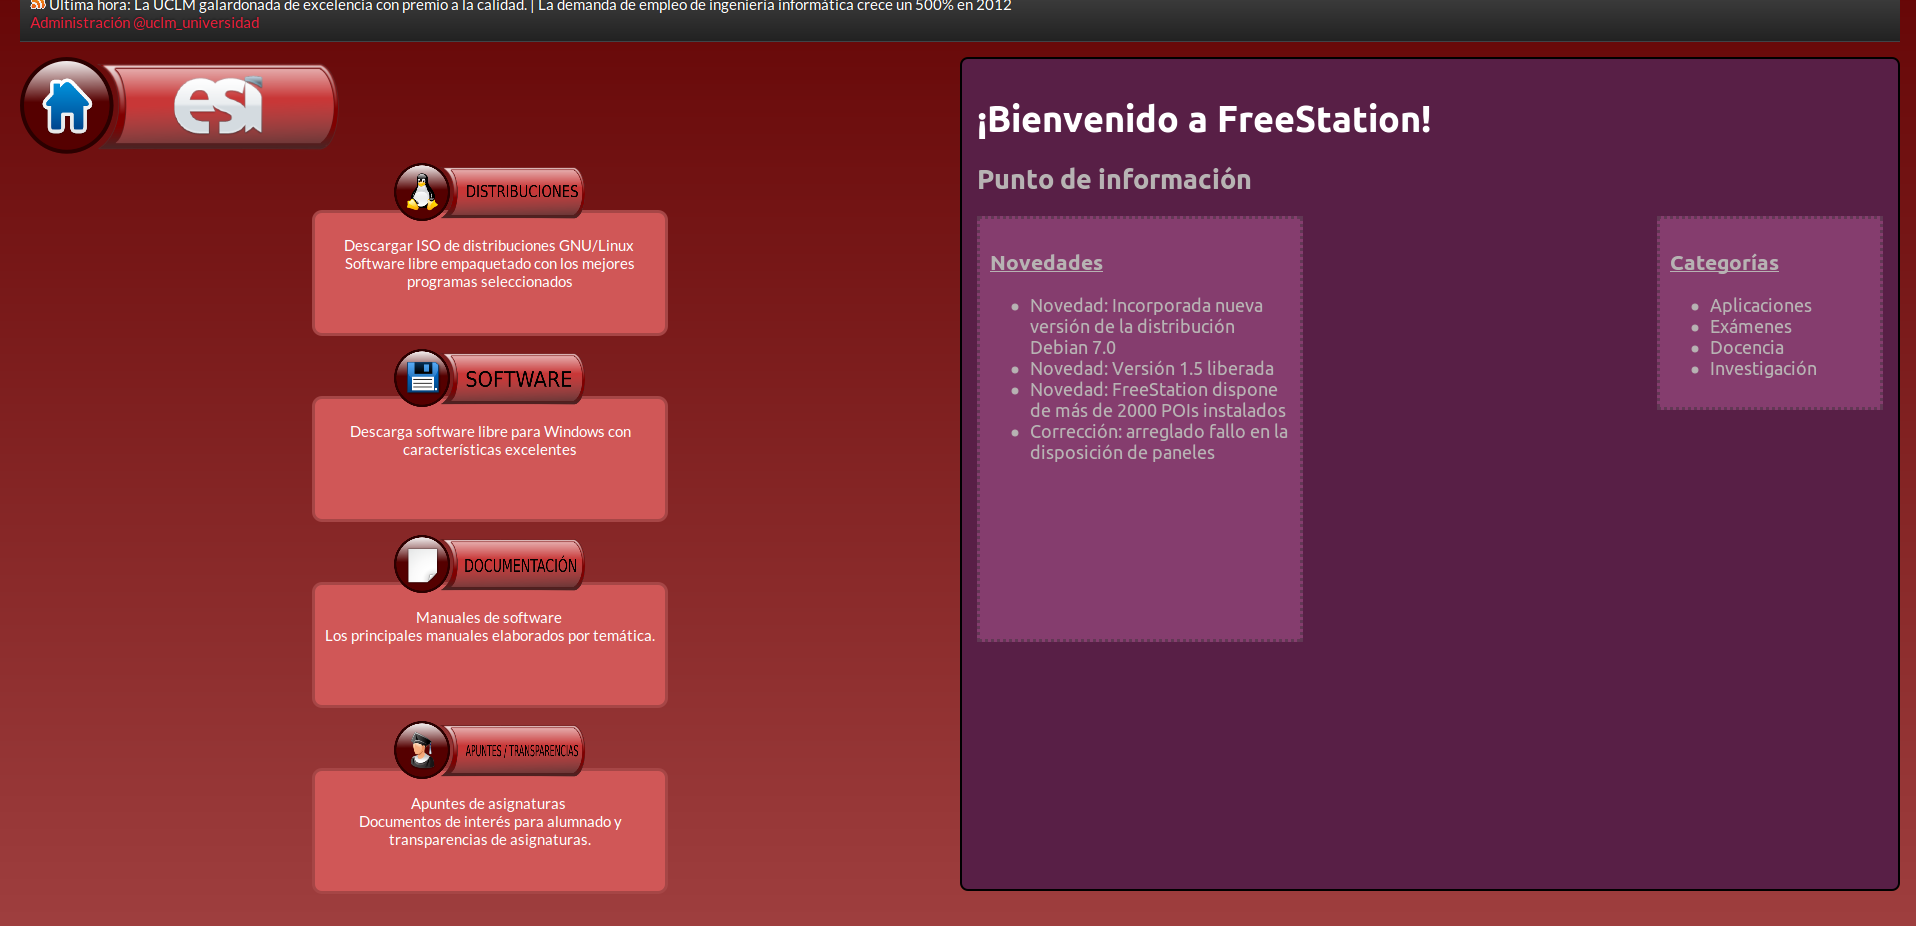
\includegraphics[width=425px]{src/img/couchdb-explotation-case1.png}
        \caption[Caso de explotación basado en CouchDB - Vista inicial] {Caso de
        explotación basado en CouchDB - Vista inicial}
        \label{fig:couchexplotationnui1}
    \end{center}
\end{figure}

La figura ~\ref{fig:couchexplotationnui1} muestra la pantalla de bienvenida
basada en estas nuevas tecnologías, que en comparación con la figura
~\ref{fig:explotationgtkinit} es notablemente superior.

\newpage

\begin{figure}[ht]
    \begin{center}
        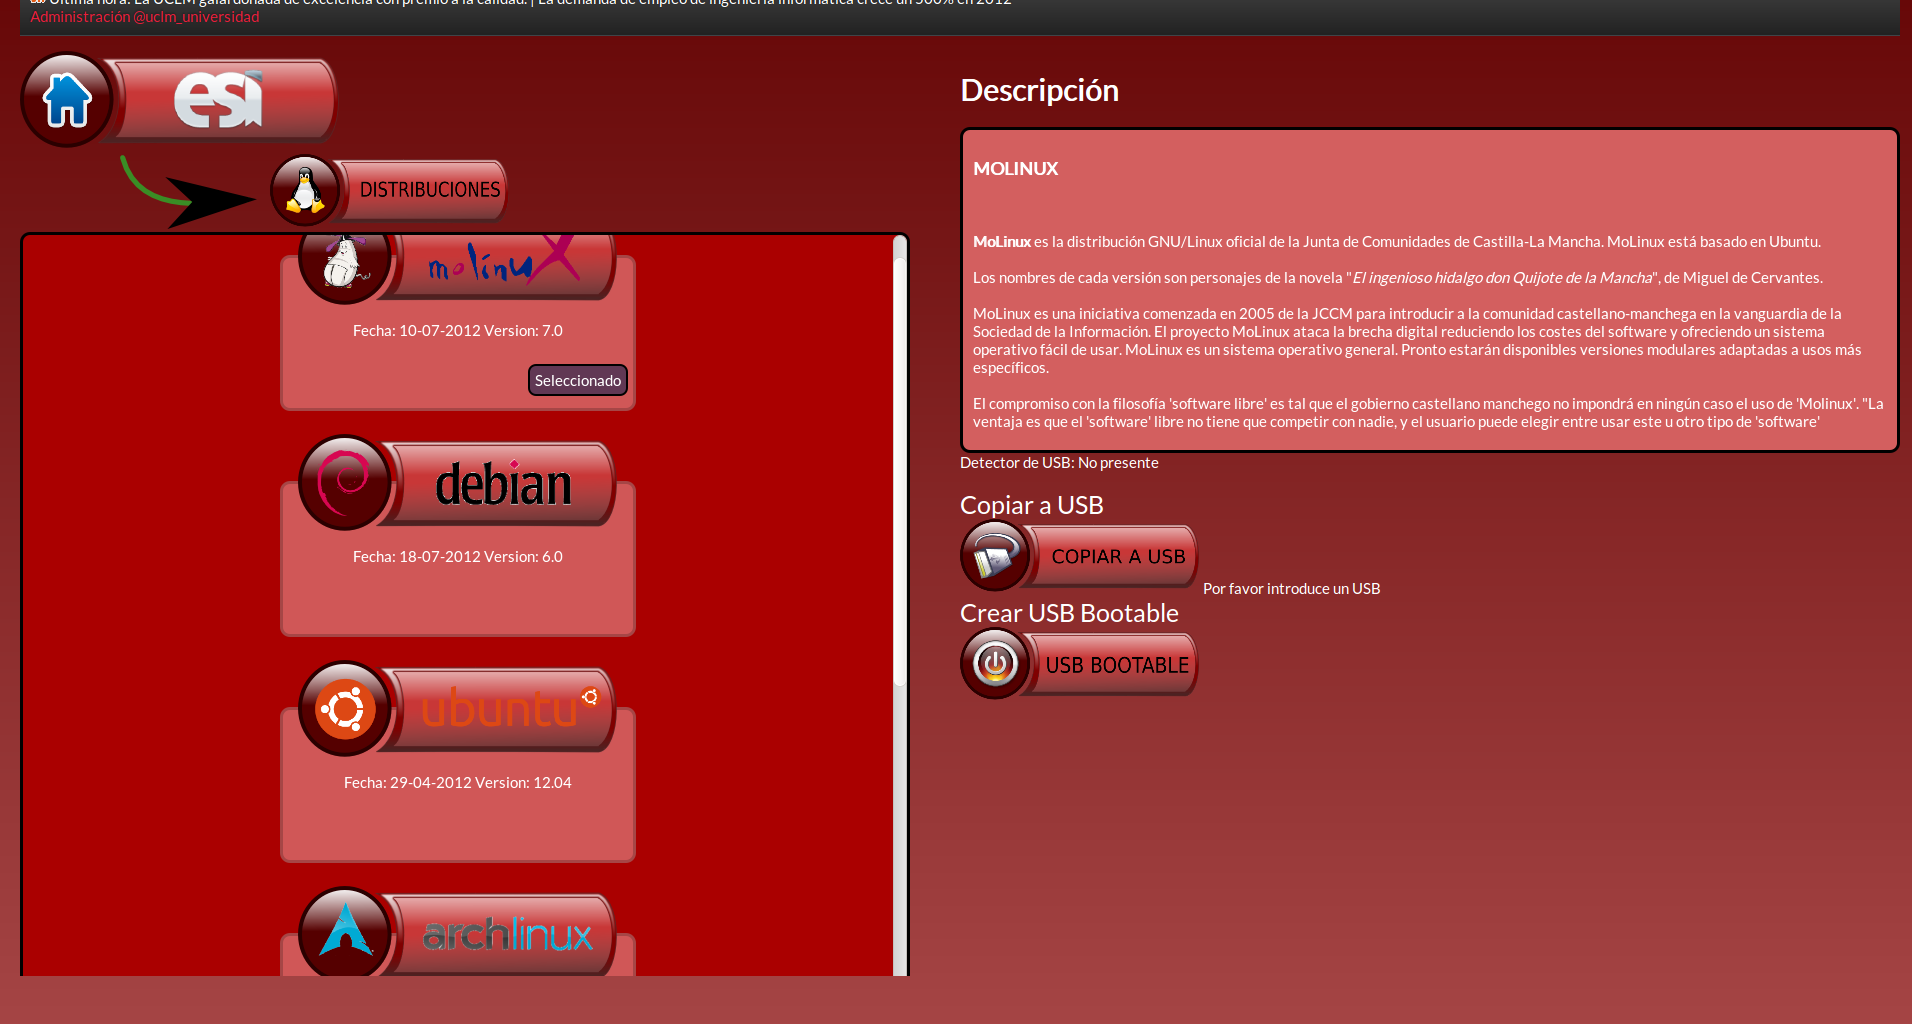
\includegraphics[width=425px]{src/img/couchdb-explotation-case2.png}
        \caption[Caso de explotación basado en CouchDB - Vista de distribuciones]
          {Caso de explotación basado en CouchDB - Vista de distribuciones}
          \label{fig:couchexplotationnui2}
    \end{center}
\end{figure}

De la misma forma, la figura ~\ref{fig:couchexplotationnui2} muestra que la 
vista de distribuciones mejoró su aparencia y fue posible añadir efectos de fade
\emph{in/fade out} que no son apreciables en las capturas de pantalla, pero 
si en ejecución de la aplicación. Los degradados lineales, border redondeados,
opacidades, etc mejoran ampliamente la visualización del efecto resultado final.

En el desarrollo se han tenido en cuenta los principios de diseño NUI se la
sección ~\ref{sec:generacionint} como por ejemplo:

\begin{itemize}
    \item \textbf{Contexto}: aprovechar el contexto como principio fundamental de
    diseño, en este caso, educativo y con entorno similar a la paleta de diseño de la UCLM.
    
    \item \textbf{Interacciones}: aprovechar interacciones NUI donde el usuario
    tendría un beneficio de interfaz. Los efectos \emph{in/fade out}, opacidad, notificación de acciones y
    remarcados de interacción contribuyen en este punto probando mejoras en las
    mecánicas fundamentales de las interacciones primarias.
    
    \item \textbf{Menos es más}: proponer un diseño simple sin pérdida de
    información y con casos de uso muy concretos.
\end{itemize}

\newpage

La incorporación de nuevas características como la internalización (que no ha
sido completada por falta de tiempo) deberían resultar triviales de añadir sobre
el caso de explotación actual. En definitiva, la acción de añadir nuevas
características a FreeStation resulta sencilla así como adaptar el interfaz a
las necesidades particulares de cada organización. Este enfoque abre multitud de
puertas abiertas al desarrollo y mejoras del proyecto.

\cleardoublepage